\documentclass[12pt,a4paper]{report}

% Encoding and Fonts
\usepackage[utf8]{inputenc}
\usepackage[T1]{fontenc}
\usepackage{times}

% Packages for Mathematics and Symbols
\usepackage{amsmath, amsfonts, amssymb}
\usepackage{bm}

% Packages for Graphics and Figures
\usepackage{graphicx}
\usepackage{float}
\usepackage{tikz}
\usetikzlibrary{arrows.meta, positioning, shapes.multipart, calc}
\usepackage{pgfgantt}
\usepackage{caption}
\usepackage{subcaption}

% Packages for Hyperlinks
\usepackage{hyperref}
\hypersetup{
    colorlinks=true,
    linkcolor=blue,
    urlcolor=blue,
    citecolor=blue
}

% Page Layout
\usepackage{geometry}
\geometry{a4paper, margin=1in}

% Header and Footer
\usepackage{fancyhdr}
\pagestyle{fancy}
\fancyhf{}
\setlength{\headheight}{26.98592pt}
\fancyhead[L]{\leftmark}
\fancyfoot[C]{\thepage}

% Section Formatting
\usepackage{titlesec}
\titleformat{\chapter}[display]
  {\normalfont\huge\bfseries\color{blue}}
  {\chaptername\ \thechapter}{20pt}{\Huge}
\titlespacing*{\chapter}{0pt}{0pt}{20pt}

% Table of Contents Formatting
\usepackage{tocloft}
\renewcommand{\cftchapfont}{\bfseries}
\renewcommand{\cftsecfont}{\bfseries}

% Bibliography
\usepackage{cite}

% Package for Algorithms
\usepackage{algorithm}
\usepackage{algorithmic}

% Package for Multirow in Tables
\usepackage{multirow}

% Package for Adjusting Table Columns
\usepackage{array}

% Line Spacing
\usepackage{setspace}
\onehalfspacing % 1.5 spacing

% Document Information
\title{\textbf{Hybrid Data Augmentation Techniques for Disease Identification from Clinical Notes}}
\author{
    \textbf{Kaustabh Ganguly} \\
    Roll Number: CH23M514 \\
    \\
    \textbf{Mentors}: \\
    Samyabrata Chakraborty \\
    Debopam Nanda \\
}
\date{November 30, 2024}

\begin{document}

% Cover Page
\begin{titlepage}
    \centering
    
\includegraphics[width=4cm]{logo.png} \\
    \vspace{0.5cm}
    {\large \bfseries M.Tech Project Report\\
    INDIAN INSTITUTE OF TECHNOLOGY MADRAS \\
    CHENNAI -- 600036} \\
    \vspace{1.5cm}
    {\huge \bfseries Hybrid Data Augmentation Techniques for Disease Identification from Clinical Notes} \\
    \vspace{2cm}
    {\Large \textit{A Project Report}} \\
    \vspace{0.5cm}
    {\large Submitted by} \\
    \vspace{0.5cm}
    {\Large \bfseries Kaustabh Ganguly} \\
    \vspace{0.5cm}
    {\large For the award of the degree of} \\
    \vspace{0.5cm}
    {\Large \bfseries MASTER OF TECHNOLOGY} \\
    \vspace{1.5cm}
    {\large \bfseries November 2024} \\
    \vfill
    {\small \textcopyright~2024 Indian Institute of Technology Madras}
\end{titlepage}

% Thesis Certificate Page
\newpage
~\vfill
\begin{center}
    \textbf{Thesis Certificate}
\end{center}
\vspace{0.5in}
This is to certify that the thesis titled \textit{``Hybrid Data Augmentation Techniques for Disease Identification from Clinical Notes''} submitted by \textbf{Kaustabh Ganguly}, Roll Number \textbf{CH23M514}, is a bona fide record of the work done under our guidance. \\

\vspace{1in}

\noindent \textbf{Mentors}: \\
Samyabrata Chakraborty \hfill Signature: \\
Debopam Nanda \hfill Signature: \\

\vfill
\newpage

% Abstract
\chapter*{Abstract}
\label{chap:abstract}

This thesis presents a novel approach to improving rare disease coverage in automated ICD coding by leveraging synthetic clinical text generation, advanced knowledge integration, and efficient computational strategies. First, it addresses the fundamental challenge of long-tail data scarcity in real-world medical records, which leads to suboptimal prediction performance for underrepresented ICD codes. To mitigate this, large language models (LLMs) are employed to produce factually grounded and diverse discharge summaries that capture realistic patient comorbidities, guided by structured medical ontologies such as SNOMED CT and Orphanet. A rigorous, multi-phase validation pipeline – combining rule-based checks for medical plausibility, LLM-based fact verification to detect subtle contradictions, and ICD feedback loops to ensure label consistency – filters out inaccurate synthetic samples. These high-quality, balanced datasets are then used to train and refine multi-label ICD classification models, including transformer-based architectures (e.g., PLM-ICD) and synonym-aware networks. Emphasis is placed on rare disease codes, with the synthetic corpus boosting their representation and improving macro-F1 and recall metrics. Addressing hardware constraints, the methodology integrates quantization (QLoRA), gradient checkpointing, and knowledge distillation so that larger models can be fine-tuned on a moderate GPU setup without sacrificing accuracy. The research further tackles error analysis, bias detection, and explainability, employing methods like attention visualization and SHAP attributions to ensure transparent, trustworthy predictions. By uniting sophisticated data augmentation, knowledge-based validation, and memory-efficient training, this work seeks to significantly advance the scalability and coverage of automated ICD coding systems, particularly for rare disorders where annotation gaps currently limit clinical AI effectiveness.


\chapter{Introduction}
\label{chap:introduction}

\section{Background}
Healthcare facilities rely on standardized coding schemes to categorize patient diagnoses, procedures, and comorbidities. The \textbf{International Classification of Diseases (ICD)}, maintained by the World Health Organization (WHO), is the most widely adopted system, with ICD-10 and ICD-11 being the modern variants \cite{who2019icd11}. In large-scale hospital databases like \textbf{MIMIC-IV}, each admission may have multiple ICD codes assigned, reflecting the patient’s primary complaint, secondary conditions, and complications.

Despite the critical importance of ICD codes in reimbursement, epidemiological monitoring, and healthcare research, accurate coding remains difficult. Assigning codes manually is labor-intensive and prone to errors, especially when dealing with long discharge summaries containing multiple, potentially rare conditions. Automation can help streamline these processes but faces key hurdles in data imbalance, complexity of clinical text, and the need for transparency in model outputs.

\section{Importance of ICD Coding}
ICD codes underpin numerous healthcare activities:
\begin{itemize}
    \item \textbf{Billing and Reimbursement:} Proper code assignments ensure fair compensation for patient care.
    \item \textbf{Clinical Research and Surveillance:} Epidemiological studies, rare-disease registries, and population-level analyses rely on coded data to identify relevant cohorts.
    \item \textbf{Hospital and Public Health Management:} Resource planning, policy-making, and outbreak detection all draw on aggregated ICD codes.
\end{itemize}
Any systemic inaccuracies in ICD assignment can thus ripple through the healthcare ecosystem, impacting finances, patient outcomes, and research quality.

\section{Challenges in Manual ICD Coding}
\begin{itemize}
    \item \textbf{High Volume and Complexity:} Large hospitals generate tens of thousands of discharge summaries, each potentially referencing multiple diagnoses and procedures.
    \item \textbf{Ambiguous or Unstructured Notes:} Clinical text frequently contains abbreviations, non-standard phrases, and domain-specific terms \cite{wrenn2010quantifying}.
    \item \textbf{Risk of Human Error:} Even experienced coders can overlook secondary or rare conditions when processing lengthy documents.
\end{itemize}
As a result, there is a growing interest in \textit{automated ICD coding} systems to improve consistency and reduce the coding burden.

\section{Need for Automated ICD Coding}
Automated solutions hold promise in:
\begin{itemize}
    \item \textbf{Enhancing Efficiency:} Minimizing the time coders spend on each patient record.
    \item \textbf{Boosting Accuracy:} Mitigating undercoding or overcoding issues, especially if advanced natural language understanding is employed.
    \item \textbf{Scaling to Large Data:} Managing databases with millions of records while retaining fidelity in code assignments.
\end{itemize}
However, practical deployment of automated ICD coding remains non-trivial—particularly for rare or complex codes.

\section{Challenges in Automated ICD Coding}
\label{sec:challenges-automated}
Past research in automated ICD coding has achieved notable success with frequent codes, yet several obstacles persist \cite{dong2022automated,edin2023automated}:
\begin{itemize}
    \item \textbf{Data Imbalance:} A small subset of common codes appears abundantly, whereas many codes (often clinically significant) occur only a handful of times \cite{rios2018few}.
    \item \textbf{Long and Redundant Notes:} Discharge summaries can exceed thousands of words, requiring efficient and effective text representations \cite{heo2022medical}.
    \item \textbf{Complex Multi-Label Task:} A single note may encode multiple diagnoses; models must handle the combinatorial explosion of possible label subsets.
    \item \textbf{Explainability and Bias:} Clinicians demand interpretable predictions to trust automated outputs \cite{holzinger2017we}, and any systemic bias in data or model training can compromise patient care.
\end{itemize}

\section{Existing Approaches and Limitations}
Early work on automated ICD coding used \textbf{rule-based} systems \cite{farkas2008automatic} or \textbf{traditional machine learning} (e.g., SVMs, logistic regression) \cite{perotte2014diagnosis}, but these often struggled to capture semantic nuances in clinical notes. More recent research has turned to:
\begin{itemize}
    \item \textbf{Neural Networks:} CNN- or RNN-based methods (e.g., CAML \cite{mullenbach2018explainable}, LAAT \cite{vu2020label}) show improved performance but still suffer on rare codes.
    \item \textbf{Transformer-Based Models:} BERT variants \cite{devlin2019bert} and specialized models (PLM-ICD \cite{huang2022plm}, ModernBERT \cite{warner2024modernbert}) can handle complex text but often require truncation for very long documents.
    \item \textbf{Curriculum Learning and Hierarchical Methods:} Some work leverages the hierarchy of ICD codes \cite{ren2022hicu}, but coverage for rare labels remains suboptimal.
\end{itemize}
Moreover, simple data-level strategies (like random oversampling) can lead to overfitting or bias, highlighting the need for domain-aware augmentation.

\section{Problem Statement}
Given the crucial role of ICD codes and the steep challenge of \textbf{rare or underrepresented conditions}, this thesis aims to develop an automated ICD coding pipeline that:
\begin{enumerate}
    \item Significantly boosts recall and precision for rarely occurring ICD codes.
    \item Maintains or improves overall performance on common codes.
    \item Provides transparent and interpretable predictions suitable for clinical review.
\end{enumerate}
The system should handle long, unstructured notes and be robust to the wide variety of clinical scenarios in MIMIC-IV.

\section{Proposed Solution}
To tackle the above challenges, we propose a holistic framework encompassing:
\begin{enumerate}
    \item \textbf{LLM-Driven Synthetic Data Generation:} Use large language models, enriched by medical ontologies (e.g., SNOMED CT, UMLS) and co-occurrence statistics, to create realistic discharge summaries for underrepresented ICD codes. A \emph{rigorous validation pipeline} filters out hallucinated or inconsistent samples.
    \item \textbf{Advanced Multi-Label Classification Architectures:} Explore CNN-based (CAML, LAAT), transformer-based (PLM-ICD, MSMN, ModernBERT), and knowledge-aware approaches (hyperbolic embeddings, retrieval augmentation) to determine optimal strategies for rare-code prediction.
    \item \textbf{Explainability and Bias Assessment:} Apply attention visualization, SHAP, or integrated gradients to interpret predictions, especially for complex or rare labels. Evaluate potential demographic or disease-specific biases introduced by synthetic data.
    \item \textbf{Environment and Resource Optimization:} Implement quantization, gradient checkpointing, and other memory-saving techniques to train large models within a 6GB GPU or Colab Pro+ constraints.
\end{enumerate}

\section{Objectives}
Key objectives include:
\begin{itemize}
    \item \textbf{Objective 1: Data Augmentation for Rare Codes.} Demonstrate that LLM-informed synthetic samples can mitigate long-tail issues and improve macro-F1 on rarely occurring diagnoses by at least 10--15\%.
    \item \textbf{Objective 2: Comprehensive Validation.} Implement a multi-layer validation approach—combining rule-based checks, LLM-based factual analysis, and retrieval-based verification—to ensure synthetic notes are both coherent and medically plausible.
    \item \textbf{Objective 3: High-Performing Classifier.} Achieve state-of-the-art or near state-of-the-art results on MIMIC-IV ICD-10 benchmarks, focusing on improved recall for difficult or rare codes.
    \item \textbf{Objective 4: Interpretability and Bias Analysis.} Provide consistent interpretability tools (e.g., code-level attention maps) and systematically analyze any performance disparities or biases introduced by synthetic data augmentation.
\end{itemize}

\section{Thesis Outline}
This thesis is organized as follows:
\begin{itemize}
    \item \textbf{Chapter 2: Literature Review} --- Surveys existing ICD coding techniques, synthetic text generation, and curriculum/hierarchical methods.
    \item \textbf{Chapter 3: Problem Definition and Formulation} --- Delves deeper into the multi-label setup, data imbalance, and the formal task setting.
    \item \textbf{Chapter 4: Methodology} --- Details the advanced data augmentation pipeline, knowledge integration, and model architectures.
    \item \textbf{Chapter 5: Dataset Understanding} --- Explores MIMIC-IV’s characteristics, focusing on code frequency distributions and note length.
    \item \textbf{Chapter 6: Results} --- Presents experimental outcomes, including ablations for synthetic data, error analysis, and bias detection.
    \item \textbf{Chapter 7: Conclusion and Work Timeline} --- Summarizes achievements, limitations, and proposes directions for future research.
\end{itemize}

In essence, this research seeks to \textbf{bridge the data imbalance gap} in ICD coding by leveraging domain-specific knowledge and advanced synthetic generation techniques. By pairing these augmented datasets with cutting-edge model architectures, we aim to achieve robust and interpretable performance gains, particularly for complex or rare diagnoses.

\section{Background}
Accurate medical coding is essential in modern healthcare systems for various purposes, including billing, epidemiology, research, and clinical decision support. The \textbf{International Classification of Diseases (ICD)} is a standardized system developed by the World Health Organization (WHO) for coding diseases, symptoms, and procedures~\cite{who2019icd11}. In particular, the latest version, \textbf{ICD-11}, provides a comprehensive coding system used globally.

\section{Importance of ICD Coding}
ICD codes serve as a critical link between clinical care and administrative functions. They are used for:
\begin{itemize}
    \item \textbf{Billing and Reimbursement}: Accurate coding ensures that healthcare providers are appropriately reimbursed for the services provided.
    \item \textbf{Clinical Research}: Researchers use ICD codes to identify patient populations and study disease prevalence and outcomes.
    \item \textbf{Public Health Surveillance}: Health authorities monitor disease outbreaks and trends using aggregated ICD code data.
    \item \textbf{Healthcare Planning}: Policy-makers rely on coding data to allocate resources and plan healthcare services.
\end{itemize}

\section{Challenges in Manual ICD Coding}
Despite its importance, manual ICD coding is a complex and time-consuming process. Trained medical coders must interpret unstructured clinical narratives and assign appropriate codes. Challenges include:
\begin{itemize}
    \item \textbf{Volume of Data}: Healthcare facilities generate vast amounts of clinical documentation daily.
    \item \textbf{Complexity of Coding Systems}: The ICD system contains thousands of codes, with ICD-10-CM having around 68,000 diagnosis codes~\cite{dong2022automated}.
    \item \textbf{Ambiguity in Clinical Language}: Clinical notes often contain ambiguous or colloquial language, making interpretation difficult.
    \item \textbf{Human Error}: Manual coding is prone to errors, which can lead to incorrect billing, compliance issues, and compromised data quality.
\end{itemize}

\section{Need for Automated ICD Coding}
To address these challenges, there is a pressing need for automated ICD coding systems that can:
\begin{itemize}
    \item \textbf{Improve Efficiency}: Reduce the time and effort required for manual coding.
    \item \textbf{Enhance Accuracy}: Minimize human errors and improve coding consistency.
    \item \textbf{Support Scalability}: Handle large volumes of clinical data efficiently.
    \item \textbf{Facilitate Data Utilization}: Enable better use of clinical data for research and decision-making.
\end{itemize}

\section{Challenges in Automated ICD Coding}
While automated ICD coding holds promise, it faces several significant challenges:
\begin{itemize}
    \item \textbf{Data Imbalance and Scarcity}: Clinical datasets exhibit a long-tailed distribution of ICD codes, with a few codes being highly frequent and many codes occurring rarely~\cite{rios2018few}. Models often perform poorly on rare codes due to insufficient training data.
    \item \textbf{Complexity of Clinical Texts}: Clinical narratives are lengthy, unstructured, and contain domain-specific terminology, abbreviations, and inconsistencies~\cite{wrenn2010quantifying}.
    \item \textbf{Multi-Label Classification}: Assigning ICD codes is a multi-label task, where multiple codes may be relevant for a single clinical note.
    \item \textbf{Explainability and Interpretability}: Healthcare professionals require transparent and interpretable models to trust and adopt automated coding systems~\cite{holzinger2017we}.
\end{itemize}

\section{Existing Approaches and Limitations}
Various machine learning and deep learning approaches have been proposed for automated ICD coding:
\begin{itemize}
    \item \textbf{Rule-Based Systems}: Early methods relied on handcrafted rules and keyword matching but lacked scalability and adaptability~\cite{farkas2008automatic}.
    \item \textbf{Traditional Machine Learning}: Techniques like Support Vector Machines and Decision Trees were used but struggled with high-dimensional, sparse data and failed to capture semantic nuances~\cite{perotte2014diagnosis}.
    \item \textbf{Deep Learning Models}: Convolutional Neural Networks (CNNs) and Recurrent Neural Networks (RNNs) have improved performance by learning hierarchical representations of text~\cite{mullenbach2018explainable, vu2020label}. However, they often underperform on rare codes due to data imbalance.
    \item \textbf{Transformer-Based Models}: Models like BERT have advanced natural language understanding but may not consistently outperform CNNs in clinical text classification and face challenges with long documents~\cite{dong2022automated, gao2021limitations}.
    \item \textbf{Curriculum Learning and Hierarchical Models}: Methods like HiCu leverage the hierarchical structure of ICD codes to improve performance on rare codes~\cite{ren2022hicu}.
\end{itemize}

Despite these advancements, significant gaps remain in effectively handling data imbalance, processing complex clinical texts, and providing explainable predictions.

\section{Problem Statement}
In this thesis, we address the problem of accurately predicting ICD codes from clinical narratives, with a focus on improving performance on rare codes. The key challenges include:
\begin{itemize}
    \item \textbf{Data Imbalance}: Handling the long-tailed distribution of ICD codes and the scarcity of annotated data for rare codes.
    \item \textbf{Complexity of Clinical Texts}: Processing lengthy and unstructured clinical narratives to extract relevant information.
    \item \textbf{Explainability}: Providing interpretable predictions to gain clinician trust.
\end{itemize}

\section{Proposed Solution}
To tackle these challenges, we propose a comprehensive approach that includes:
\begin{itemize}
    \item \textbf{Hybrid Data Augmentation}: Combining Retrieval Augmented Generation (RAG) with ontology-based methods to generate synthetic clinical notes for rare diseases, augmenting the training data.
    \item \textbf{Knowledge Integration}: Leveraging medical ontologies and knowledge graphs (e.g., SNOMED CT, RxNorm) to enrich data representation and model understanding of medical concepts.
    \item \textbf{Transformer-Based Models}: Utilizing advanced transformer architectures adapted for long clinical documents to capture contextual information.
    \item \textbf{Multi-Label Classification Techniques}: Implementing label embedding, hierarchical classification, and label grouping to handle the extensive label space.
    \item \textbf{Explainability Techniques}: Integrating methods like SHAP, LIME, and Integrated Gradients to provide transparent insights into model predictions.
\end{itemize}

\section{Objectives}
The objectives of this thesis are:
\begin{enumerate}
    \item Develop an advanced, explainable model for ICD code prediction, focusing on rare codes.
    \item Implement hybrid data augmentation techniques to address data imbalance.
    \item Integrate medical knowledge through ontologies and knowledge graphs.
    \item Enhance model interpretability to facilitate clinical acceptance.
\end{enumerate}

\section{Thesis Outline}
The remainder of this thesis is organized as follows.
\begin{itemize}
    \item \textbf{Chapter 2: Literature Review} – A detailed review of existing approaches and challenges in automated ICD coding.
    \item \textbf{Chapter 3: Definition and formulation of the problem} – A precise statement of the problem and its formulation.
    \item \textbf{Chapter 4: Methodology} – An in-depth explanation of the proposed methods and details of the implementation.
    \item \textbf{Chapter 5: Dataset Understanding} – A description of the datasets used and their characteristics.
    \item \textbf{Chapter 6: Results} – Presentation and analysis of the experimental results.
    \item \textbf{Chapter 7: Conclusion and Work Timeline} – A summary of the work and the plan for completing the remaining tasks.
\end{itemize}

\chapter{Literature Review}

The automation of the International Classification of Diseases (ICD) coding process has emerged as a critical area of research in medical informatics and Natural Language Processing (NLP). The ICD is a globally recognized system used for classifying diseases and health conditions, essential for epidemiological studies, health management, and clinical billing. Manual ICD coding involves assigning appropriate codes to clinical narratives, a task that is both time-consuming and prone to errors due to the complexity and volume of medical records. The transition from ICD-9 to ICD-10 and now to ICD-11 has further increased the complexity, with a significant expansion in the number of codes and granularity~\cite{who2019icd11}.

\section{Early Approaches to Automated ICD Coding}

Early approaches to automate ICD coding primarily relied on rule-based systems and traditional machine learning techniques. Rule-based methods utilized handcrafted rules, regular expressions, and keyword matching to map clinical terms to ICD codes~\cite{farkas2008automatic, scheurwegs2017data}. While these approaches achieved high precision in specific contexts, they lacked scalability and adaptability to the extensive and evolving ICD code sets. The complexity and dynamic nature of classification systems, such as ICD-10-CM with around 68,000 diagnosis codes~\cite{dong2022automated}, posed significant challenges for rule-based systems to cover all possible coding scenarios.

Traditional machine learning methods, such as Support Vector Machines (SVMs) and Decision Trees, employed feature engineering to represent clinical texts numerically~\cite{perotte2014diagnosis}. These methods often required extensive preprocessing and could not effectively capture the semantic richness of clinical narratives. Moreover, they struggled with high-dimensional and sparse data characteristic of clinical texts and did not generalize well to unseen or rare codes.

\section{Deep Learning in Automated ICD Coding}

The advent of deep learning has revolutionized NLP by enabling models to learn hierarchical and abstract representations of text data without extensive feature engineering~\cite{lecun2015deep}. In the context of automated ICD coding, deep learning models have been employed to effectively capture complex patterns in clinical narratives and improve coding accuracy.

\subsection{Convolutional and Recurrent Neural Networks}

Convolutional Neural Networks (CNNs) have been applied to capture local syntactic and semantic patterns in text~\cite{kim2014convolutional}. Mullenbach et al.~\cite{mullenbach2018explainable} introduced the Convolutional Attention for Multi-Label classification (CAML) model, which employs a convolutional encoder followed by a label-wise attention mechanism. The attention mechanism allows the model to focus on relevant parts of the text for each ICD code, enhancing interpretability. The attention weights for each label $l$ are computed as:

\begin{equation}
\alpha^{(l)} = \text{softmax}(W^{(l)} h + b^{(l)}),
\end{equation}

where $h$ represents the hidden representations from the convolutional layers, and $W^{(l)}$, $b^{(l)}$ are the label-specific parameters.

Building upon CAML, Li and Yu~\cite{li2020multi} proposed the Multi-Filter Residual Convolutional Neural Network (MultiResCNN), which integrates residual connections and multiple convolutional filters to capture patterns at various granularities. The model enhances feature extraction and improves performance on the ICD coding task.

Recurrent Neural Networks (RNNs), particularly Long Short-Term Memory (LSTM) networks, have been utilized to capture sequential dependencies in clinical texts~\cite{hochreiter1997long}. Vu et al.~\cite{vu2020label} introduced the Label-Attention model (LAAT), which employs a bidirectional LSTM encoder and a structured self-attention mechanism to generate label-specific document representations. The attention mechanism in LAAT is formulated as:

\begin{equation}
A = \text{softmax}(U \tanh(P H)),
\end{equation}

where $H$ is the sequence of hidden states from the bidirectional LSTM, $P$ is a projection matrix, and $U$ is a label embedding matrix. The label-specific representations are then used to predict the ICD codes.

While these models have shown improvements over traditional methods, they still face limitations. CNNs, for instance, may not effectively capture long-range dependencies due to their local receptive fields. RNNs can model sequences but suffer from issues like vanishing gradients and computational inefficiency with long texts. Additionally, both CNNs and RNNs may struggle with the extensive label space and data imbalance inherent in ICD coding tasks.

\subsection{Transformer-Based Models}

Transformer-based models, such as BERT~\cite{devlin2019bert}, have further advanced the field by enabling models to capture long-range dependencies and contextual information through self-attention mechanisms. Huang et al.~\cite{huang2022plm} proposed the PLM-ICD model, which leverages pre-trained language models for the ICD coding task. The PLM-ICD model integrates a pre-trained BERT encoder with a label attention mechanism, allowing it to benefit from large-scale language pre-training and focus on relevant text segments for each code.

However, an empirical observation is that current BERT-based approaches do not consistently achieve better performance than CNN-based methods for multi-label classification applied to clinical coding~\cite{dong2022automated, gao2021limitations}. This limitation may be attributed to the inefficiency of BERT in modeling concept-level information and handling long clinical documents. Gao et al.~\cite{gao2021limitations} highlighted that BERT's fixed input length and computational complexity make it less suitable for processing lengthy discharge summaries without truncation, potentially leading to information loss.

Heo et al.~\cite{heo2022medical} addressed the challenge of applying BERT to long clinical documents by introducing the Document-to-Sequence BERT (D2SBERT) model. D2SBERT divides lengthy discharge summaries into multiple sequences of fixed length and processes each sequence independently using BERT. They then apply a sequence attention mechanism to capture important information across these sequences for ICD code prediction. Their experiments on the MIMIC-III dataset demonstrated that D2SBERT outperforms previous models, including CNN-based methods, in predicting ICD codes.

\subsection{Modern BERT-Based Encoders for ICD Coding}
Recently, there has been renewed interest in optimizing BERT-based encoders specifically for efficient inference and long-context processing in the medical coding domain. Several works propose modern architectures that extend BERT and incorporate domain-specific pretraining or architectural innovations:

\begin{itemize}
    \item \textbf{MosaicBERT}~\cite{portes2023mosaicbert} and \textbf{CrammingBERT}~\cite{geiping2023cramming}: Focus on training efficiency and matching BERT performance with shorter training times. Although these methods accelerate training, they do not necessarily improve performance for very long clinical narratives.

    \item \textbf{NomicBERT}~\cite{nussbaum2024nomicbert} and \textbf{GTE-en-MLM}~\cite{zhang2024gte}: Emphasize long-context capabilities (e.g., 2048 to 8192 tokens) and partial improvements for retrieval tasks. They also employ new data splits or advanced unpadding approaches, yet they still rely on older BERT-based designs that can be memory-intensive.

    \item \textbf{ModernBERT}~\cite{warner2024modernbert}: A recently introduced bidirectional encoder that implements architectural modifications (e.g., alternating local-global attention, RoPE embeddings, label attention modules) designed for speed and memory efficiency up to 8192 tokens. ModernBERT outperforms many previous baselines on short and long context ICD coding benchmarks, suggesting that a hardware-aware design can achieve state-of-the-art performance while drastically reducing inference cost.
\end{itemize}

These modernized BERT-like encoders demonstrate that carefully tailoring model architecture and pretraining strategies for clinical data---particularly addressing long-sequence challenges and domain vocabulary---can yield significant gains in speed, memory efficiency, and accuracy. However, they still face the common limitation of data imbalance for rare codes, indicating that novel data augmentation or hierarchical training approaches remain crucial.

\subsection{Curriculum Learning and Hierarchical Models}

Curriculum learning is a training strategy where models are exposed to training examples in a meaningful order, generally from easy to hard, to improve learning efficiency and performance~\cite{bengio2009curriculum}. In the context of automated ICD coding, the hierarchical structure of ICD codes presents an opportunity to apply curriculum learning by leveraging the relationships among codes.

Ren et al.~\cite{ren2022hicu} introduced Hierarchical Curriculum Learning (HiCu), an algorithm that utilizes the hierarchical structure of ICD codes to create a curriculum for multi-label classification models. HiCu constructs a label tree from the ICD code hierarchy and trains the model in a sequence of rounds, each focusing on a different level of the hierarchy. At each round, the model learns to predict codes at a particular level before proceeding to more specific codes in the next level.

The HiCu algorithm employs a knowledge transfer mechanism using hyperbolic embeddings to initialize model parameters for each level based on the parameters from the previous level. This approach ensures that the model builds upon previously learned representations, facilitating the learning of more complex and specific codes.

By integrating curriculum learning with hierarchical knowledge, HiCu aims to improve model generalization, particularly for rare and less frequent codes. Their experiments on the MIMIC-III dataset showed that HiCu significantly improves predictive performance across different neural architectures, including CNNs, RNNs, and transformer-based models. The method resulted in higher macro-AUC and macro-F1 scores, indicating better performance on rare codes.

HiCu addresses the challenge of data imbalance by emphasizing the hierarchical relationships among labels and gradually increasing the difficulty of the learning task. This method demonstrates the potential of curriculum learning and hierarchical modeling in enhancing automated ICD coding systems.

\section{Challenges in Automated ICD Coding}

Despite these advancements, automated ICD coding faces several significant challenges, as detailed by Dong et al.~\cite{dong2022automated}, Edin et al.~\cite{edin2023automated}, and Nguyen et al.~\cite{nguyen2023mimicivicd}.

\subsection{Data Imbalance and Scarcity}

One of the primary issues is data imbalance and scarcity, particularly for rare ICD codes. Clinical datasets exhibit a long-tailed distribution of codes, where a few codes are highly frequent, and many codes occur rarely. In the MIMIC-III dataset~\cite{johnson2016mimic}, for example, around 5,000 codes appear fewer than 10 times in the training data, and over 50\% of codes never appear~\cite{rios2018few}. This imbalance leads to models that perform well on frequent codes but poorly on rare ones. Handling unseen, infrequent, and imbalanced labels is a key problem for multi-label classification with many labels.

Edin et al.~\cite{edin2023automated} conducted a critical review and replicability study, finding that models underperform on rare codes due to weak configurations, poorly sampled train-test splits, and insufficient evaluation. They corrected the calculation of the macro F1-score, which had been sub-optimally computed in previous studies due to the inclusion of codes missing from the test set. Their revised evaluation doubled the macro F1-scores and provided a more accurate assessment of model performance on rare codes.

Nguyen et al.~\cite{nguyen2023mimicivicd} highlighted that MIMIC-IV includes both ICD-9 and ICD-10 codes, with significantly more documents and unique labels compared to MIMIC-III. They discussed the challenges posed by the long-tailed distribution of ICD codes in MIMIC-IV, where the majority of codes are rare. By evaluating existing methods under more extreme conditions with longer-tailed distributions and a higher number of ICD codes, they provided a more comprehensive assessment of model performance.

Ren et al.~\cite{ren2022hicu} addressed data imbalance by leveraging the hierarchical structure of ICD codes in a curriculum learning framework. By training models to predict codes at different levels of the hierarchy sequentially, their HiCu algorithm improves performance on rare codes, as demonstrated by higher macro-AUC and macro-F1 scores.

\subsection{Processing Long and Complex Clinical Documents}

Clinical narratives, such as discharge summaries, can be lengthy and contain redundant or irrelevant information, often referred to as "note bloat"~\cite{wrenn2010quantifying}. Models may struggle to identify the relevant information for each code within such documents. However, Edin et al.~\cite{edin2023automated} conducted an error analysis and found that document length had only a negligible impact on overall model performance, suggesting that other factors, such as code frequency, play a more significant role.

Heo et al.~\cite{heo2022medical} proposed D2SBERT to address the challenge of processing long clinical documents. By dividing documents into manageable sequences and applying a sequence attention mechanism, D2SBERT effectively captures important information across the entire document without truncating it. This approach allows transformer-based models to handle long texts and improves ICD code prediction accuracy.

\subsection{Explainability and Interpretability}

Explainability and interpretability are crucial in healthcare applications, as clinicians need to understand the rationale behind model predictions to trust and effectively use automated systems~\cite{holzinger2017we}. While attention mechanisms provide some level of interpretability by highlighting relevant text segments, the highlighted texts mostly indicate associations instead of causality. Further studies are needed to evaluate the usefulness of highlights for clinical coders and to integrate more inherently explainable methods, such as incorporating symbolic representations of the coding steps with deep learning.

Edin et al.~\cite{edin2024unsupervised} proposed an unsupervised approach to achieve supervised-level explainability in healthcare records. They introduced adversarial robustness training to improve explanation plausibility and proposed a new explanation method, AttInGrad, which combines attention and gradient-based attributions. Their method produces explanations of comparable quality to supervised approaches without the need for costly evidence-span annotations.

Ren et al.~\cite{ren2022hicu} utilized hyperbolic embeddings and knowledge transfer mechanisms in their HiCu algorithm, which not only improves predictive performance but also provides insights into the hierarchical relationships among ICD codes. By structuring the learning process according to the ICD code hierarchy, their method enhances interpretability by aligning the model's learning trajectory with the established medical coding system.

\section{Embedding Models and Clinical Semantic Search}

The effectiveness of embedding models in medical semantic search tasks is critical for various applications, including document retrieval and information extraction. Excoffier et al.~\cite{excoffier2024generalist} compared generalist embedding models with specialized clinical embedding models in a semantic search task using rephrased ICD-10-CM code descriptions. Their results showed that generalist models performed better than clinical models, suggesting that specialized models may be more sensitive to small changes in input that confuse them.

The study highlighted that generalist models, trained on larger and more diverse datasets, may have a more robust language understanding, even in clinical contexts. This finding is significant because it challenges the assumption that domain-specific models always outperform generalist models in specialized tasks. It suggests that the training data's diversity and quantity play a crucial role in model robustness and performance.

Heo et al.~\cite{heo2022medical} demonstrated the effective use of BERT-based models in the clinical domain by adapting the model to handle long documents through sequence attention. Their approach shows that transformer-based models can be effectively applied to clinical text classification tasks when appropriately modified to address domain-specific challenges.

\section{Integrating Knowledge-Based Methods and Synthetic Data Generation}

To address the limitations of current deep learning approaches, integrating knowledge-based methods and symbolic reasoning has been proposed~\cite{dong2022automated}. Knowledge graphs and medical ontologies, such as SNOMED CT, RxNorm, and UMLS, can provide structured semantic information that enhances data representation and captures relationships between medical concepts.

Studies have explored embedding-based approaches to incorporate knowledge graphs into deep learning models~\cite{teng2020explainable, xie2019ehr}. For example, Teng et al.~\cite{teng2020explainable} utilized knowledge graphs to enhance the explainability and performance of ICD coding models by integrating semantic information from medical ontologies.

Ren et al.~\cite{ren2022hicu} employed hyperbolic embeddings to capture the hierarchical structure of ICD codes in their HiCu algorithm. Hyperbolic embeddings are effective in representing hierarchical data due to their ability to model tree-like structures in a continuous space with low distortion~\cite{nickel2017poincare}. By incorporating hyperbolic embeddings, HiCu leverages the ICD code hierarchy to improve model performance and interpretability.

Synthetic data generation has emerged as a promising approach to address data scarcity and imbalance in medical coding tasks. The generation of synthetic clinical notes can augment existing datasets, particularly for rare diseases, and enhance model performance.

Kumichev et al.~\cite{kumichev2024medsyn} introduced \textit{MedSyn}, a medical text generation framework that integrates large language models (LLMs) with a Medical Knowledge Graph (MKG). By sampling prior medical information from the MKG and generating synthetic clinical notes using GPT-4 and fine-tuned LLaMA models, they demonstrated that synthetic data could increase the classification accuracy of vital and challenging ICD codes by up to 17.8\% compared to settings without synthetic data.

\section{Summary of Literature Review}

Automated ICD coding is a promising application of AI in healthcare, offering potential improvements in efficiency and accuracy of the coding process. However, significant challenges remain, including handling data imbalance, processing long and complex documents, integrating symbolic reasoning, and ensuring explainability. Combining deep learning with knowledge-based methods, curriculum learning, and synthetic data generation, as well as involving clinical coders in the development process, are critical steps toward addressing these challenges.

Recent studies have emphasized the importance of innovative methodologies, standardized benchmarks, replicable experimental setups, and rigorous evaluation methods in automated ICD coding research. By addressing replicability issues, providing open-source code and data processing pipelines, and exploring novel data augmentation techniques, they facilitate fair comparisons and accelerate progress in the field.

Future research should focus on developing models that effectively integrate domain knowledge, handle rare and unseen codes, and provide transparent and explainable predictions. The integration of curriculum learning, advanced transformer models adapted for long clinical documents, and synthetic data generation holds promise for addressing data scarcity and enhancing model performance. Additionally, leveraging generalist embedding models in clinical tasks may improve robustness and effectiveness in semantic search applications. By addressing the technical and organizational challenges, automated clinical coding systems can be developed and deployed to support coding in the next five years and beyond.


\chapter{Problem Definition and Formulation}

\section{Problem Statement}
The primary goal of this research is to develop an automated system that accurately predicts \textbf{ICD codes} from unstructured \textbf{clinical narratives}, with a specific focus on improving prediction performance for \textbf{rare codes}.

\section{Challenges Addressed}
The problem encompasses several challenges:
\begin{itemize}
    \item \textbf{Data Imbalance}: The ICD code distribution is highly imbalanced, with rare codes having insufficient training examples.
    \item \textbf{Complexity of Clinical Texts}: Clinical narratives are lengthy, unstructured, and contain domain-specific language.
    \item \textbf{Multi-Label Classification}: Each clinical note may correspond to multiple ICD codes, requiring effective multi-label prediction.
    \item \textbf{Knowledge Integration}: Incorporating domain knowledge from medical ontologies to enhance model understanding.
    \item \textbf{Explainability}: Providing interpretable predictions to ensure clinical trust and acceptance.
\end{itemize}

\section{Problem Formulation}
Let \( D = \{(x_i, Y_i)\}_{i=1}^N \) denote the dataset, where \( x_i \) is the \( i \)-th clinical note and \( Y_i \subseteq \mathcal{L} \) is the set of ICD codes assigned to \( x_i \), with \( \mathcal{L} \) being the set of all ICD codes.

Our objective is to learn a function \( f: X \rightarrow 2^{\mathcal{L}} \) that maps a clinical note \( x \in X \) to a subset of ICD codes \( Y \subseteq \mathcal{L} \), such that \( f \) maximizes prediction accuracy, especially for rare codes.

\section{Handling Data Imbalance}
To address data imbalance, we aim to augment the dataset \( D \) by generating synthetic clinical notes \( \tilde{x}_j \) for rare ICD codes \( l \in \mathcal{L}_{\text{rare}} \), where \( \mathcal{L}_{\text{rare}} \subseteq \mathcal{L} \) denotes the set of rare codes. This involves creating a new set \( \tilde{D} = \{(\tilde{x}_j, Y_j)\} \) to supplement the original dataset, where \( Y_j \) includes rare codes.

\section{Knowledge Integration}
We seek to enrich the model's understanding by integrating knowledge from medical ontologies \( \mathcal{O} \) (e.g., SNOMED CT, RxNorm). This involves mapping clinical entities in \( x_i \) to concepts in \( \mathcal{O} \) and using this structured information in model training. Let \( \phi(x_i) \) denote the mapping from clinical notes to ontology concepts.

\section{Multi-Label Classification Approach}
Given the large label space and hierarchical relationships among ICD codes, we plan to employ advanced multi-label classification techniques:
\begin{itemize}
    \item \textbf{Label Embedding}: Representing ICD codes in a continuous space to capture semantic relationships.
    \item \textbf{Hierarchical Classification}: Leveraging the hierarchical structure of ICD codes to inform the classification process.
    \item \textbf{Label Grouping}: Grouping similar labels to reduce complexity and improve model efficiency.
\end{itemize}

\section{Evaluation Metrics}
To evaluate the performance of the model, especially on rare codes, we will use metrics that consider class imbalance:
\begin{itemize}
    \item \textbf{Macro F1-Score}: Calculated by averaging F1-scores across all labels, giving equal weight to rare and frequent codes.
    \item \textbf{F2-Score}: Emphasizes recall over precision, aligning with the need to reduce false negatives in medical coding.
\end{itemize}

\section{Specific Goals}
Our specific goals are:
\begin{enumerate}
    \item Achieve at least a 10\% improvement in macro F2-score on rare ICD codes compared to baseline models.
    \item Generate high-quality synthetic clinical notes for rare codes using hybrid data augmentation techniques.
    \item Integrate explainability methods to provide interpretable predictions acceptable to clinicians.
\end{enumerate}

\section{Constraints and Considerations}
\begin{itemize}
    \item \textbf{Data Privacy}: Ensure compliance with data use agreements and patient privacy regulations.
    \item \textbf{Computational Resources}: Optimize model design to work within available computational resources.
    \item \textbf{Clinical Relevance}: Engage with medical experts to validate the clinical plausibility of generated notes and model predictions.
\end{itemize}

\chapter{Dataset Understanding}

\section{Overview of MIMIC-IV}
The \textbf{Medical Information Mart for Intensive Care (MIMIC-IV)} is a large, freely accessible electronic health record (EHR) dataset developed by the Beth Israel Deaconess Medical Center (BIDMC) and the Massachusetts Institute of Technology (MIT). It spans clinical stays from 2008 to 2019 and contains comprehensive, de-identified data on hospital admissions, including demographics, clinical notes, laboratory values, prescriptions, and billing codes~\cite{johnson2023mimicivscidata,nguyen2023mimicivicd}. Key modules include:
\begin{itemize}
    \item \texttt{hosp}: Hospital-wide data (e.g., \texttt{admissions}, \texttt{patients}, \texttt{diagnoses\_icd}).
    \item \texttt{icu}: ICU-specific charting data (e.g., \texttt{chartevents}).
    \item \texttt{ed}: Emergency department data.
    \item \texttt{note}: De-identified textual notes, including \texttt{discharge}.
    \item \texttt{cxr}: Linking data for chest X-ray images (MIMIC-CXR).
\end{itemize}
For automated ICD coding from discharge summaries, we focus on:
\begin{itemize}
    \item \texttt{patients} (in \textit{hosp}) for demographics (\texttt{anchor\_age}, \texttt{anchor\_year\_group}).
    \item \texttt{admissions} (in \textit{hosp}) for hospital-stay details (\texttt{hadm\_id}, \texttt{admittime}, \texttt{dischtime}).
    \item \texttt{diagnoses\_icd} (in \textit{hosp}) for billed ICD-9 or ICD-10 diagnoses.
    \item \texttt{discharge} (in \textit{note}) for textual discharge summaries.
\end{itemize}

\vspace{0.2cm}
\noindent
Below, we highlight key \textbf{SQL queries} run on \texttt{DuckDB}, their \textbf{results}, and \textbf{plots} illustrating the dataset's characteristics.

\section{Key SQL Queries and Results}

\subsection{Patient and Admission Counts}
\begin{verbatim}
SELECT
    COUNT(*) AS total_rows_in_patients,
    COUNT(DISTINCT subject_id) AS num_unique_patients
FROM mimic.patients;
\end{verbatim}
\begin{center}
\begin{tabular}{l|l}
\hline
\texttt{total\_rows\_in\_patients} & \texttt{num\_unique\_patients} \\
\hline
364627 & 364627 \\
\hline
\end{tabular}
\end{center}
So there are \textbf{364,627 unique patients} in the \texttt{patients} table.

\begin{verbatim}
SELECT
    COUNT(*) AS total_rows_in_admissions,
    COUNT(DISTINCT hadm_id) AS num_unique_admissions
FROM mimic.admissions;
\end{verbatim}
\begin{center}
\begin{tabular}{l|l}
\hline
\texttt{total\_rows\_in\_admissions} & \texttt{num\_unique\_admissions} \\
\hline
546028 & 546028 \\
\hline
\end{tabular}
\end{center}
Hence, \textbf{546,028 unique admissions} exist in MIMIC-IV.

\subsection{Multiple Admissions per Patient}
\begin{verbatim}
SELECT subject_id, COUNT(*) AS num_admissions
FROM mimic.admissions
GROUP BY subject_id
HAVING COUNT(*) > 1
ORDER BY num_admissions DESC
LIMIT 5;
\end{verbatim}
\begin{center}
\begin{tabular}{l|l}
\hline
\texttt{subject\_id} & \texttt{num\_admissions} \\
\hline
15496609 & 238 \\
15464144 & 185 \\
10714009 & 163 \\
16662316 & 142 \\
14394983 & 138 \\
\hline
\end{tabular}
\end{center}
Some patients have very frequent hospital stays (\(>100\) admissions).

\subsection{Discharge Summaries}
\begin{verbatim}
SELECT COUNT(*) AS total_discharge_notes
FROM mimic.discharge;
\end{verbatim}
\begin{center}
\begin{tabular}{l}
\hline
\texttt{total\_discharge\_notes} \\
\hline
331793 \\
\hline
\end{tabular}
\end{center}
Thus, \textbf{331,793 discharge summaries} are available.

\begin{verbatim}
SELECT
    (SELECT COUNT(DISTINCT hadm_id) FROM mimic.admissions) AS total_admissions,
    (SELECT COUNT(DISTINCT hadm_id) FROM mimic.discharge)  AS hadm_with_discharge,
    (SELECT COUNT(DISTINCT hadm_id) FROM mimic.admissions
     WHERE hadm_id NOT IN (
         SELECT DISTINCT hadm_id FROM mimic.discharge
     )
    ) AS hadm_without_discharge;
\end{verbatim}
\begin{center}
\begin{tabular}{l|l|l}
\hline
\texttt{total\_admissions} & \texttt{hadm\_with\_discharge} & \texttt{hadm\_without\_discharge} \\
\hline
546028 & 331793 & 214296 \\
\hline
\end{tabular}
\end{center}
Hence \(\sim214{,}296\) admissions have no final discharge note.

\subsection{Word Count in Discharge Summaries}
\begin{verbatim}
SELECT
    PERCENTILE_CONT(0.5)
        WITHIN GROUP (ORDER BY (LENGTH(text) - LENGTH(REPLACE(text, ' ', '')) + 1))
      AS median_word_count,
    PERCENTILE_CONT(0.9)
      WITHIN GROUP (ORDER BY (LENGTH(text) - LENGTH(REPLACE(text, ' ', '')) + 1))
    AS p90_word_count,
    PERCENTILE_CONT(0.99)
    WITHIN GROUP (ORDER BY (LENGTH(text) - LENGTH(REPLACE(text, ' ', '')) + 1))
    AS p99_word_count
FROM mimic.discharge;
\end{verbatim}
\begin{center}
\begin{tabular}{l|l|l}
\hline
\texttt{median\_word\_count} & \texttt{p90\_word\_count} & \texttt{p99\_word\_count} \\
\hline
1556 & 2556 & 3986 \\
\hline
\end{tabular}
\end{center}
Median discharge notes contain \textbf{\(\approx1{,}556\) words}, with 1\% of notes exceeding \(\approx3{,}986\) words.

\subsection{ICD-9 vs. ICD-10}
\begin{verbatim}
SELECT
    icd_version,
    COUNT(*) AS code_assignments
FROM mimic.diagnoses_icd
GROUP BY icd_version
ORDER BY code_assignments DESC;
\end{verbatim}
\begin{center}
\begin{tabular}{l|l}
\hline
\texttt{icd\_version} & \texttt{code\_assignments} \\
\hline
10 & 3455747 \\
9  & 2908741 \\
\hline
\end{tabular}
\end{center}
We have \(\sim3.46\)M ICD-10 assignments and \(\sim2.91\)M ICD-9.

\begin{verbatim}
SELECT icd_code, COUNT(*) AS freq
FROM mimic.diagnoses_icd
WHERE icd_version = 10
GROUP BY icd_code
ORDER BY freq DESC
LIMIT 10;
\end{verbatim}
\begin{center}
\begin{tabular}{l|l}
\hline
\texttt{icd\_code} & \texttt{freq} \\
\hline
E785   & 84570  \\
I10    & 83775  \\
Z87891 & 62806  \\
K219   & 56157  \\
F329   & 41876  \\
I2510  & 41550  \\
F419   & 38911  \\
N179   & 35884  \\
Z20822 & 33113  \\
Z7901  & 30957  \\
\hline
\end{tabular}
\end{center}
Common chronic diseases like hyperlipidemia (\texttt{E785}) and hypertension (\texttt{I10}) appear most frequently.

\subsection{Unique Codes and Rare-Code Challenge}
\begin{verbatim}
SELECT icd_version,
       COUNT(DISTINCT icd_code) AS num_unique_codes
FROM mimic.diagnoses_icd
GROUP BY icd_version;
\end{verbatim}
\begin{center}
\begin{tabular}{l|l}
\hline
\texttt{icd\_version} & \texttt{num\_unique\_codes} \\
\hline
10 & 19440 \\
9  & 9143  \\
\hline
\end{tabular}
\end{center}
MIMIC-IV has \textbf{19,440 ICD-10 codes}. Many are rare:

\begin{verbatim}
WITH code_counts AS (
    SELECT icd_code, COUNT(*) AS freq
    FROM mimic.diagnoses_icd
    WHERE icd_version = 10
    GROUP BY icd_code
)
SELECT COUNT(*) AS codes_under_5_occurrences
FROM code_counts
WHERE freq < 5;
\end{verbatim}
\begin{center}
\begin{tabular}{l}
\hline
\texttt{codes\_under\_5\_occurrences} \\
\hline
9217 \\
\hline
\end{tabular}
\end{center}
Thus, \(\approx9{,}217\) ICD-10 codes appear fewer than 5 times (long-tail distribution).

\subsection{Average Number of ICD-10 Codes per Admission}
\begin{verbatim}
WITH code_counts AS (
    SELECT hadm_id,
           COUNT(DISTINCT icd_code) AS code_count
    FROM mimic.diagnoses_icd
    WHERE icd_version = 10
    GROUP BY hadm_id
)
SELECT AVG(code_count) AS avg_icd10_codes_per_adm
FROM code_counts;
\end{verbatim}
\begin{center}
\begin{tabular}{l}
\hline
\texttt{avg\_icd10\_codes\_per\_adm} \\
\hline
13.584911371704203 \\
\hline
\end{tabular}
\end{center}
On average, \(\sim13.6\) ICD-10 codes per admission.

\section{Visual Exploration of Data}

\begin{figure}[ht!]
    \centering
    \begin{subfigure}{0.42\textwidth}
        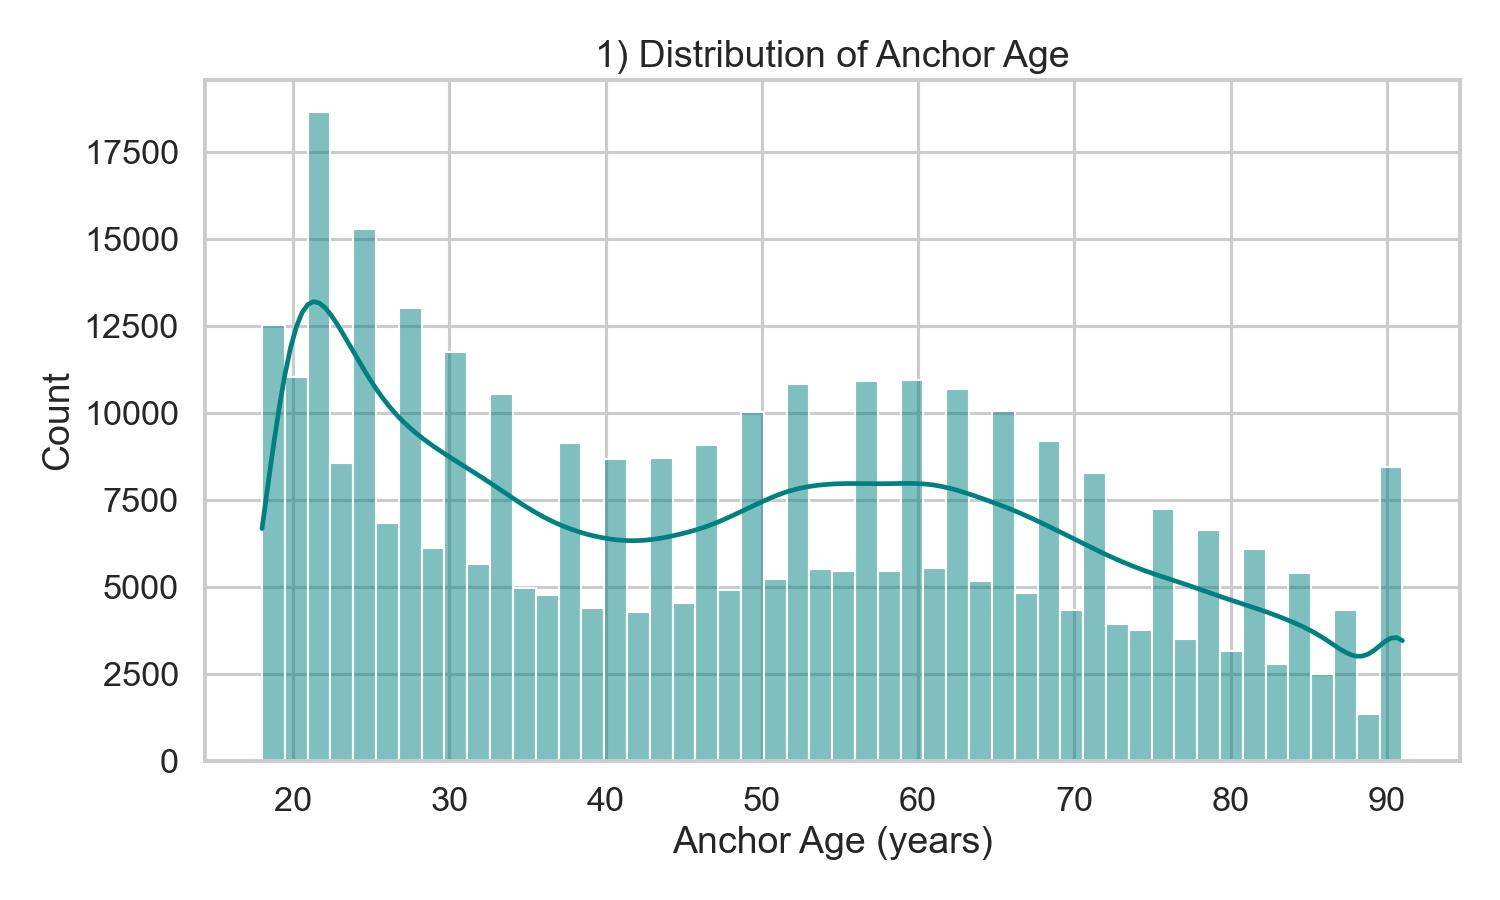
\includegraphics[width=\linewidth]{mimic_plots/plot1.jpg}
    \end{subfigure}\hfill
    \begin{subfigure}{0.54\textwidth}
        \footnotesize
        \textbf{(1) Distribution of Anchor Age}\newline
        1) The histogram shows a right-skewed age distribution, with more patients in their 20s and 30s.\newline
        2) KDE overlay highlights ages up to the capped 91 group.\newline
        3) Frequency gradually declines after middle age, with a small uptick around 90--91.
    \end{subfigure}
    \caption{Left: Distribution of Anchor Age. Right: Description.}
    \label{fig:plot1}
\end{figure}

\begin{figure}[ht!]
    \centering
    \begin{subfigure}{0.42\textwidth}
        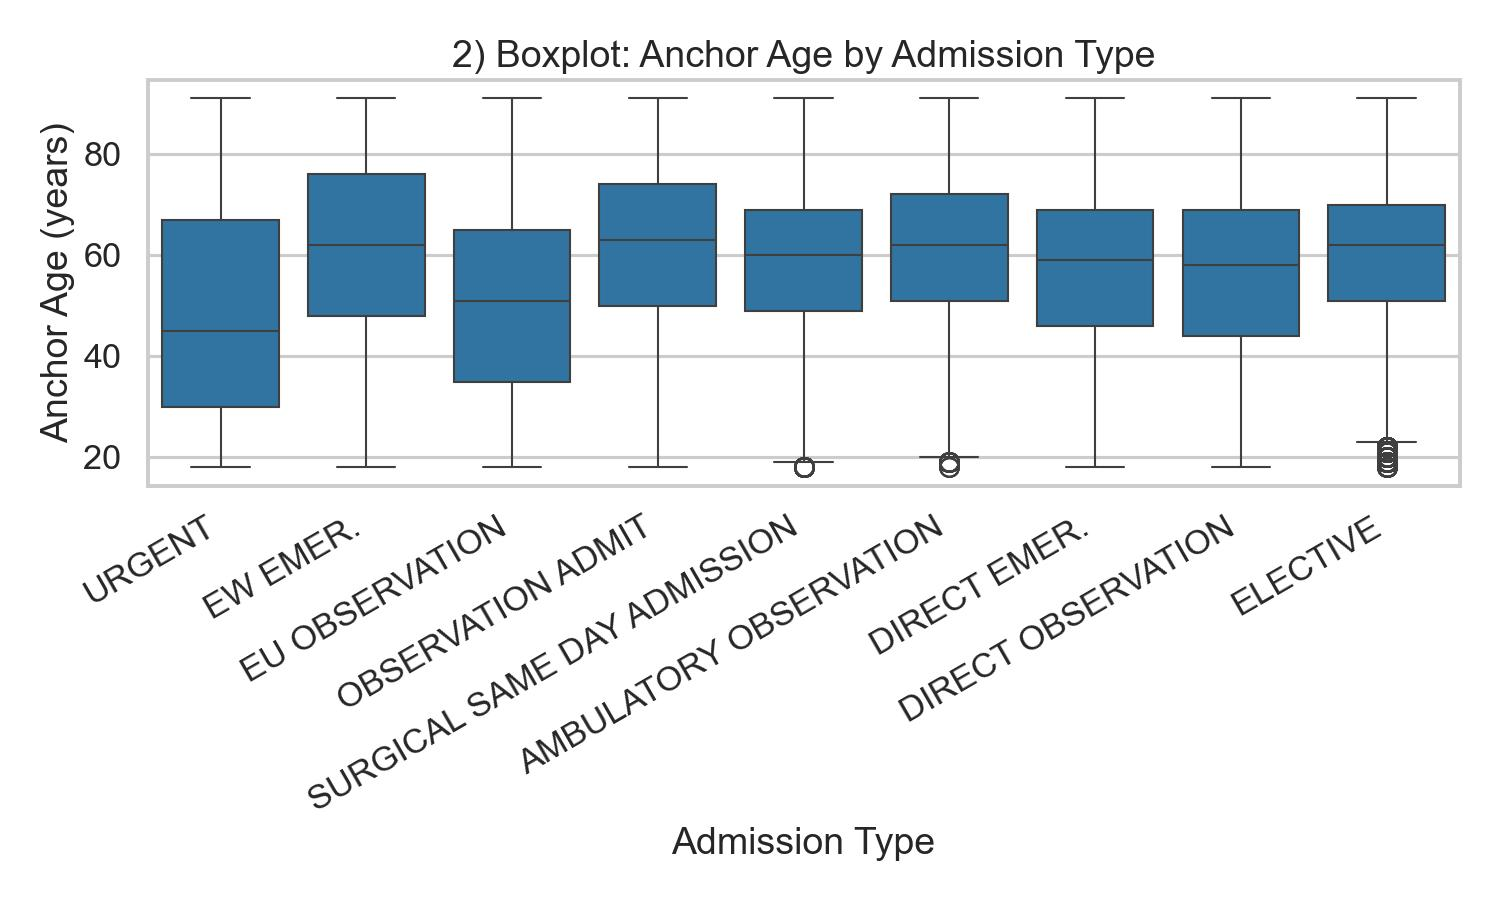
\includegraphics[width=\linewidth]{mimic_plots/plot2.jpg}
    \end{subfigure}\hfill
    \begin{subfigure}{0.54\textwidth}
        \footnotesize
        \textbf{(2) Boxplot: Anchor Age by Admission Type}\newline
        1) Shows median and spread of anchor age across each admission type.\newline
        2) Some types (e.g. “EW EMER.”) cover a broader range, while “ELECTIVE” is narrower.\newline
        3) Outliers appear as points, indicating unusual or extreme anchor ages for some admissions.
    \end{subfigure}
    \caption{Left: Boxplot for Anchor Age vs. Admission Type. Right: Description.}
    \label{fig:plot2}
\end{figure}

\begin{figure}[ht!]
    \centering
    \begin{subfigure}{0.42\textwidth}
        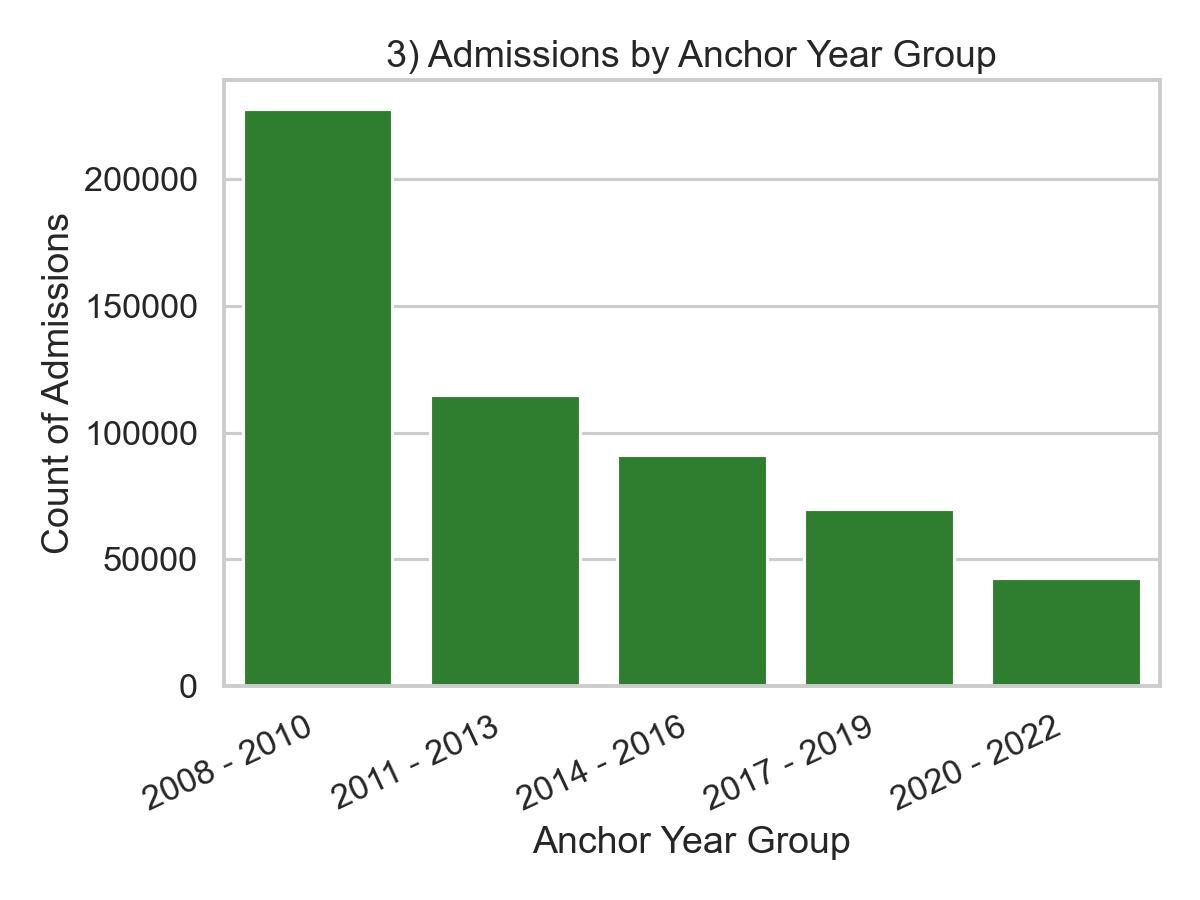
\includegraphics[width=\linewidth]{mimic_plots/plot3.jpg}
    \end{subfigure}\hfill
    \begin{subfigure}{0.54\textwidth}
        \footnotesize
        \textbf{(3) Admissions by Anchor Year Group}\newline
        1) A bar chart capturing the count of admissions over 5 approximate time intervals.\newline
        2) 2008--2010 and 2011--2013 are noticeably higher, possibly reflecting data coverage.\newline
        3) Later intervals show fewer admissions, hinting at different data capture or hospital volumes.
    \end{subfigure}
    \caption{Left: Admissions distribution by anchor year group. Right: Description.}
    \label{fig:plot3}
\end{figure}

\begin{figure}[ht!]
    \centering
    \begin{subfigure}{0.42\textwidth}
        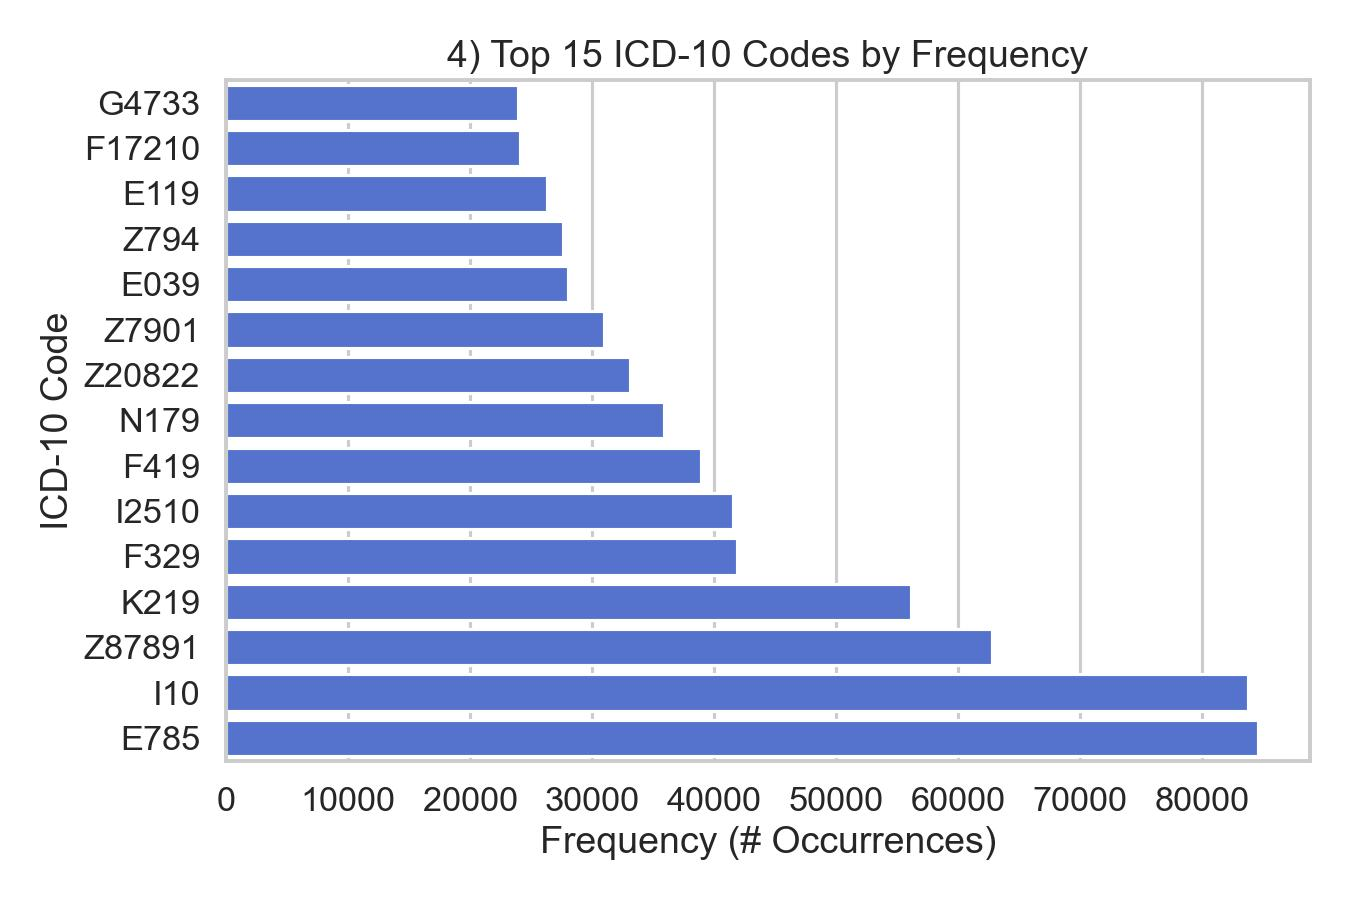
\includegraphics[width=\linewidth]{mimic_plots/plot4.jpg}
    \end{subfigure}\hfill
    \begin{subfigure}{0.54\textwidth}
        \footnotesize
        \textbf{(4) Top 15 ICD-10 Codes by Frequency}\newline
        1) Horizontal bar chart listing the most frequent ICD-10 codes.\newline
        2) E785 (Hyperlipidemia) and I10 (Hypertension) top the chart.\newline
        3) Chronic conditions like diabetes (E119) also feature prominently.
    \end{subfigure}
    \caption{Left: Bar plot of top 15 ICD-10 codes. Right: Description.}
    \label{fig:plot4}
\end{figure}

\begin{figure}[ht!]
    \centering
    \begin{subfigure}{0.42\textwidth}
        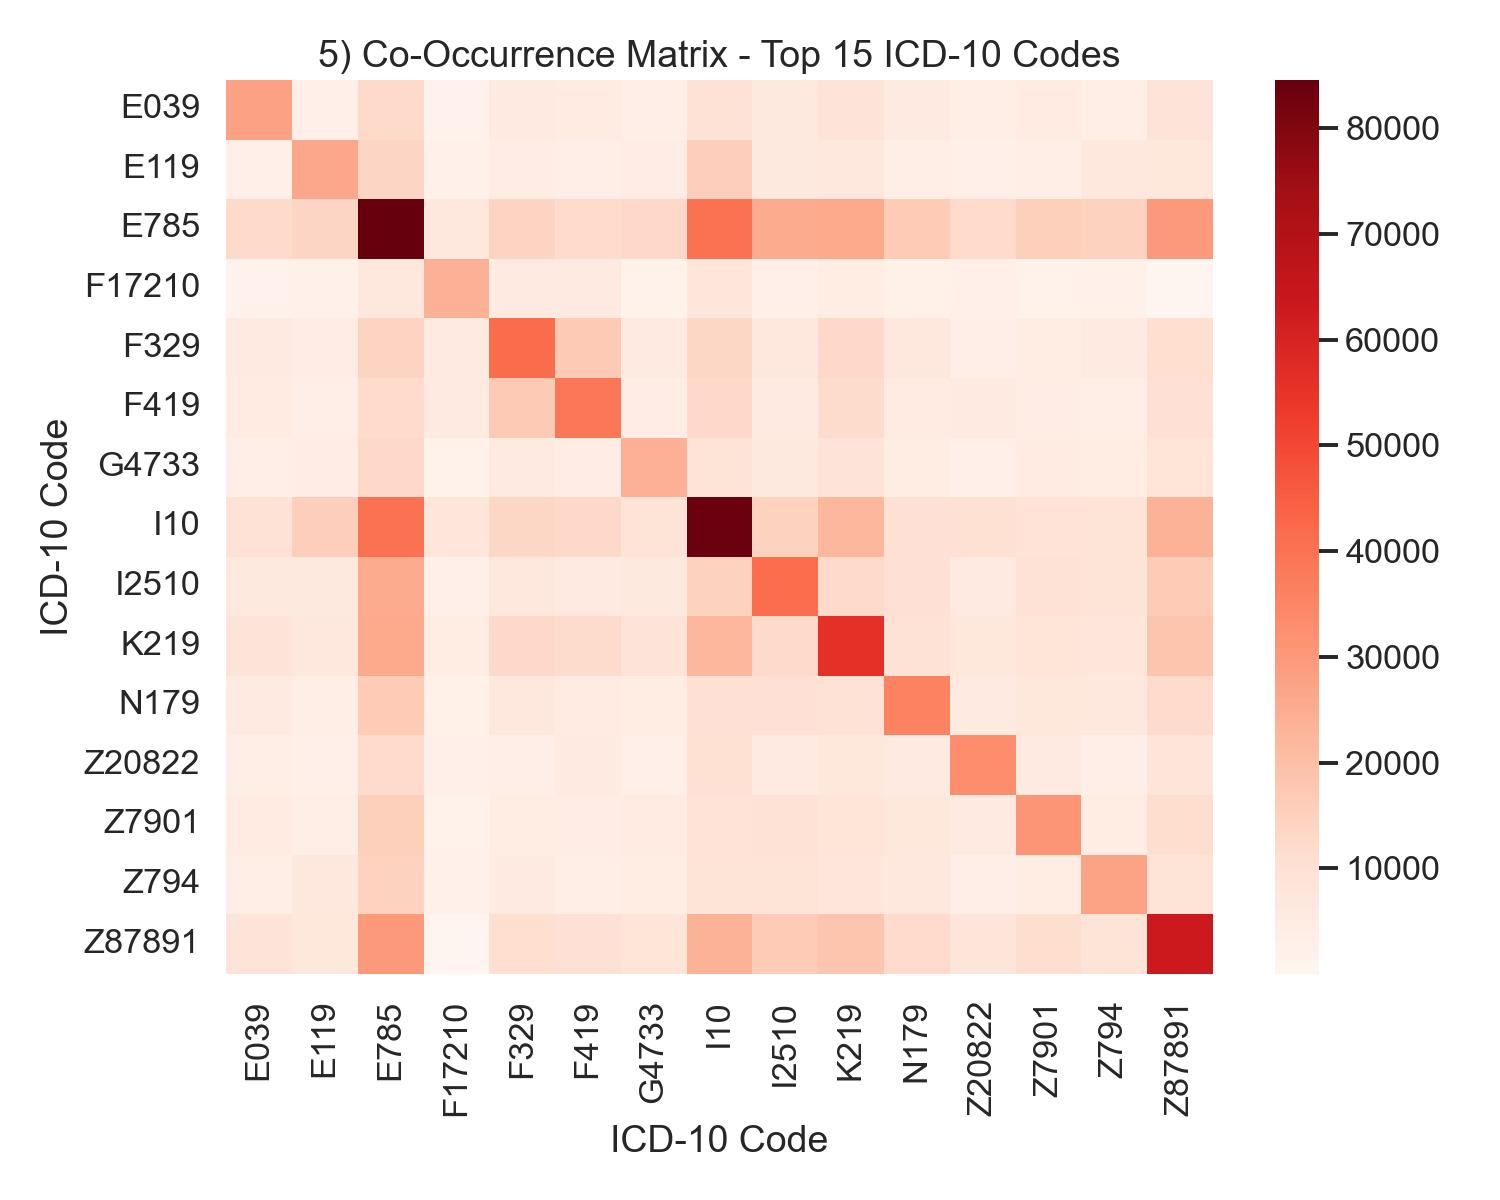
\includegraphics[width=\linewidth]{mimic_plots/plot5.jpg}
    \end{subfigure}\hfill
    \begin{subfigure}{0.54\textwidth}
        \footnotesize
        \textbf{(5) Co-Occurrence Matrix -- Top 15 ICD-10 Codes}\newline
        1) Heatmap showing how often two specific codes appear together.\newline
        2) Darker squares indicate strong co-occurrence (e.g., E785 with I10).\newline
        3) Points to common comorbidity clusters among high-frequency codes.
    \end{subfigure}
    \caption{Left: Heatmap of code co-occurrences. Right: Description.}
    \label{fig:plot5}
\end{figure}

\begin{figure}[ht!]
    \centering
    \begin{subfigure}{0.42\textwidth}
        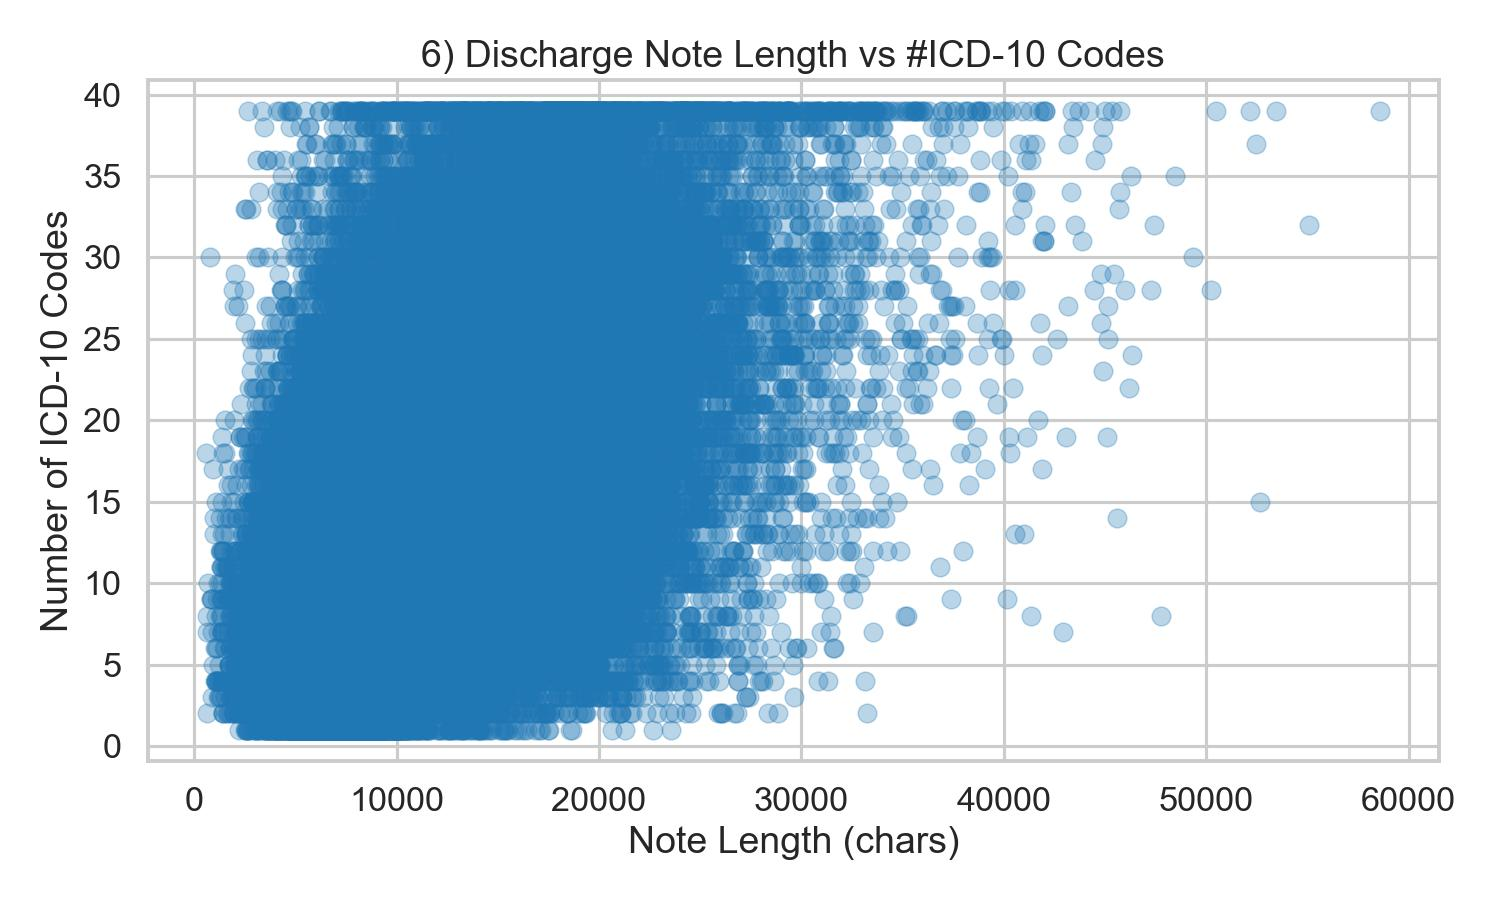
\includegraphics[width=\linewidth]{mimic_plots/plot6.jpg}
    \end{subfigure}\hfill
    \begin{subfigure}{0.54\textwidth}
        \footnotesize
        \textbf{(6) Discharge Note Length vs. \# ICD-10 Codes}\newline
        1) A scatterplot comparing how many codes an admission has vs. note length (chars).\newline
        2) There's a positive trend: very long notes often have 20+ codes.\newline
        3) The bulk of admissions cluster below 20k characters but still can have 5--15 codes.
    \end{subfigure}
    \caption{Left: Scatterplot of note length vs. number of ICD-10 codes. Right: Description.}
    \label{fig:plot6}
\end{figure}

\begin{figure}[ht!]
    \centering
    \begin{subfigure}{0.42\textwidth}
        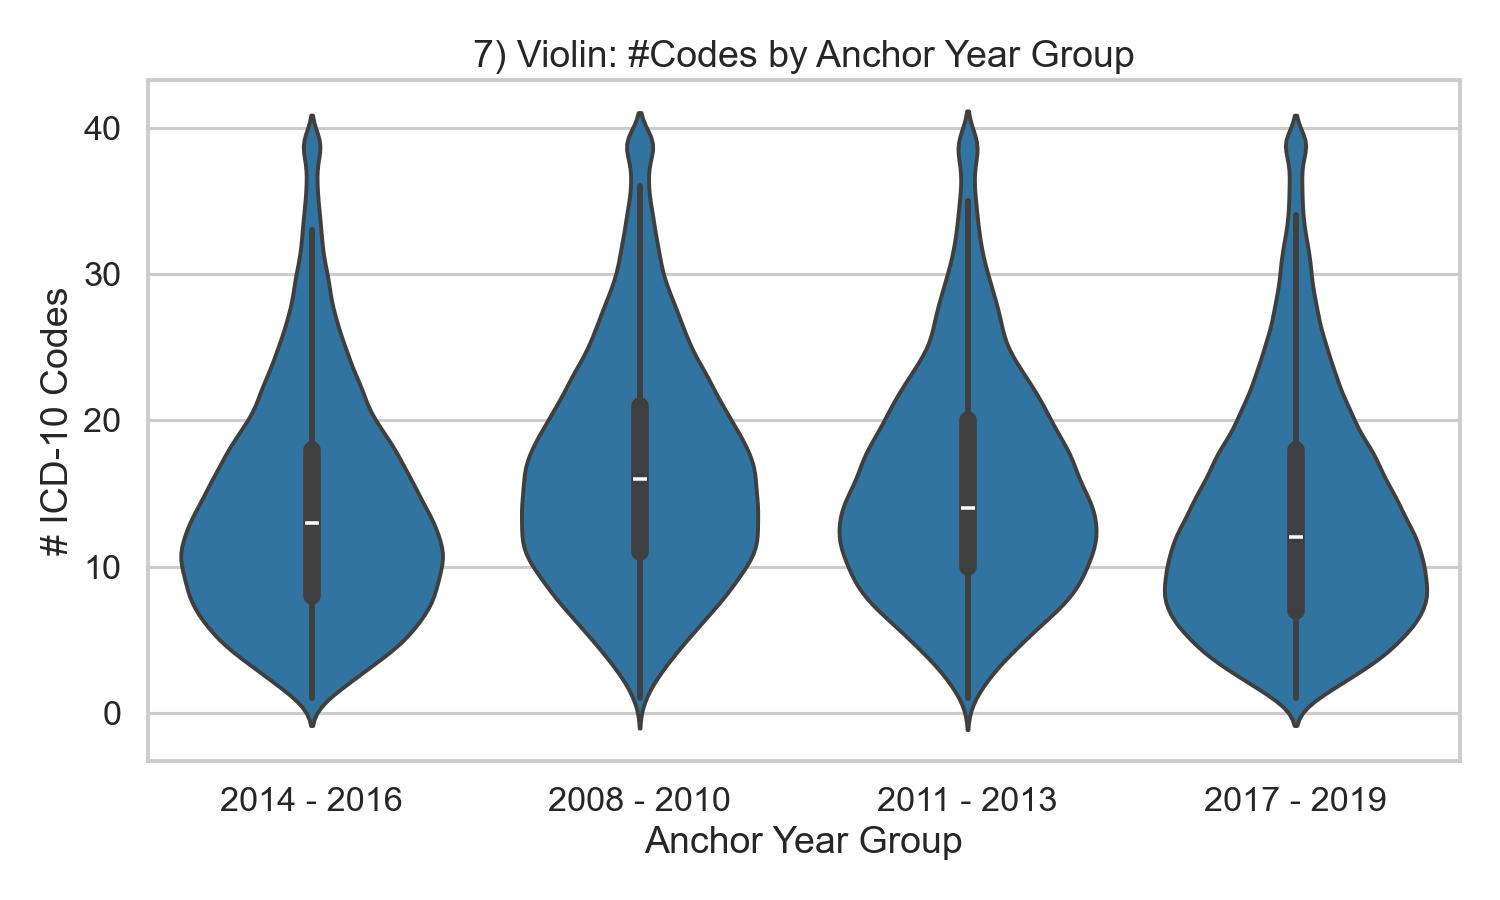
\includegraphics[width=\linewidth]{mimic_plots/plot7.jpg}
    \end{subfigure}\hfill
    \begin{subfigure}{0.54\textwidth}
        \footnotesize
        \textbf{(7) Violin: \# Codes by Anchor Year Group}\newline
        1) Violin plots indicate distribution shapes of code counts for each year group.\newline
        2) The median is shown by a white dot; thick black bar is the IQR.\newline
        3) Some groups exhibit very wide “tails,” reflecting occasional high-code admissions.
    \end{subfigure}
    \caption{Left: Violin plot of code counts across anchor year groups. Right: Description.}
    \label{fig:plot7}
\end{figure}

\begin{figure}[ht!]
    \centering
    \begin{subfigure}{0.42\textwidth}
        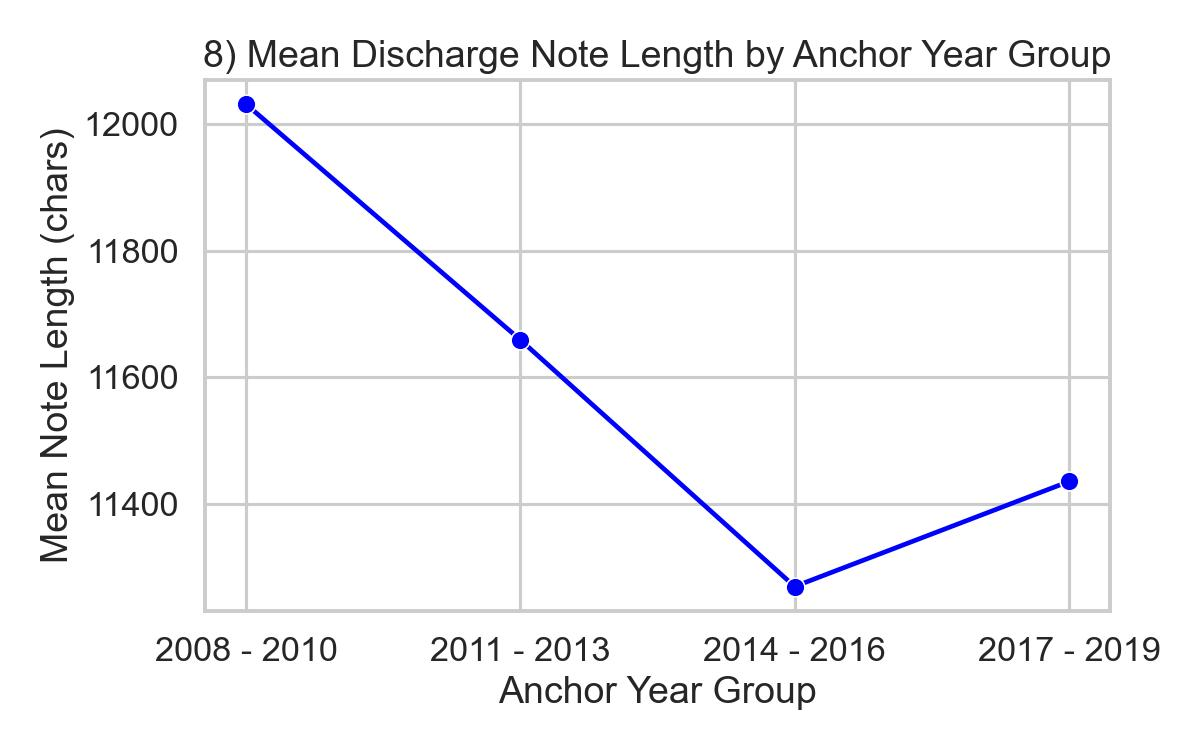
\includegraphics[width=\linewidth]{mimic_plots/plot8.jpg}
    \end{subfigure}\hfill
    \begin{subfigure}{0.54\textwidth}
        \footnotesize
        \textbf{(8) Mean Discharge Note Length by Anchor Year Group}\newline
        1) A line plot tracking average note length over time intervals.\newline
        2) Highest in 2008--2010, dipping by 2014--2016, then slight rebound.\newline
        3) Suggests evolving documentation practices or EHR usage over the years.
    \end{subfigure}
    \caption{Left: Line plot of average note length vs. anchor year group. Right: Description.}
    \label{fig:plot8}
\end{figure}

\begin{figure}[ht!]
    \centering
    \begin{subfigure}{0.42\textwidth}
        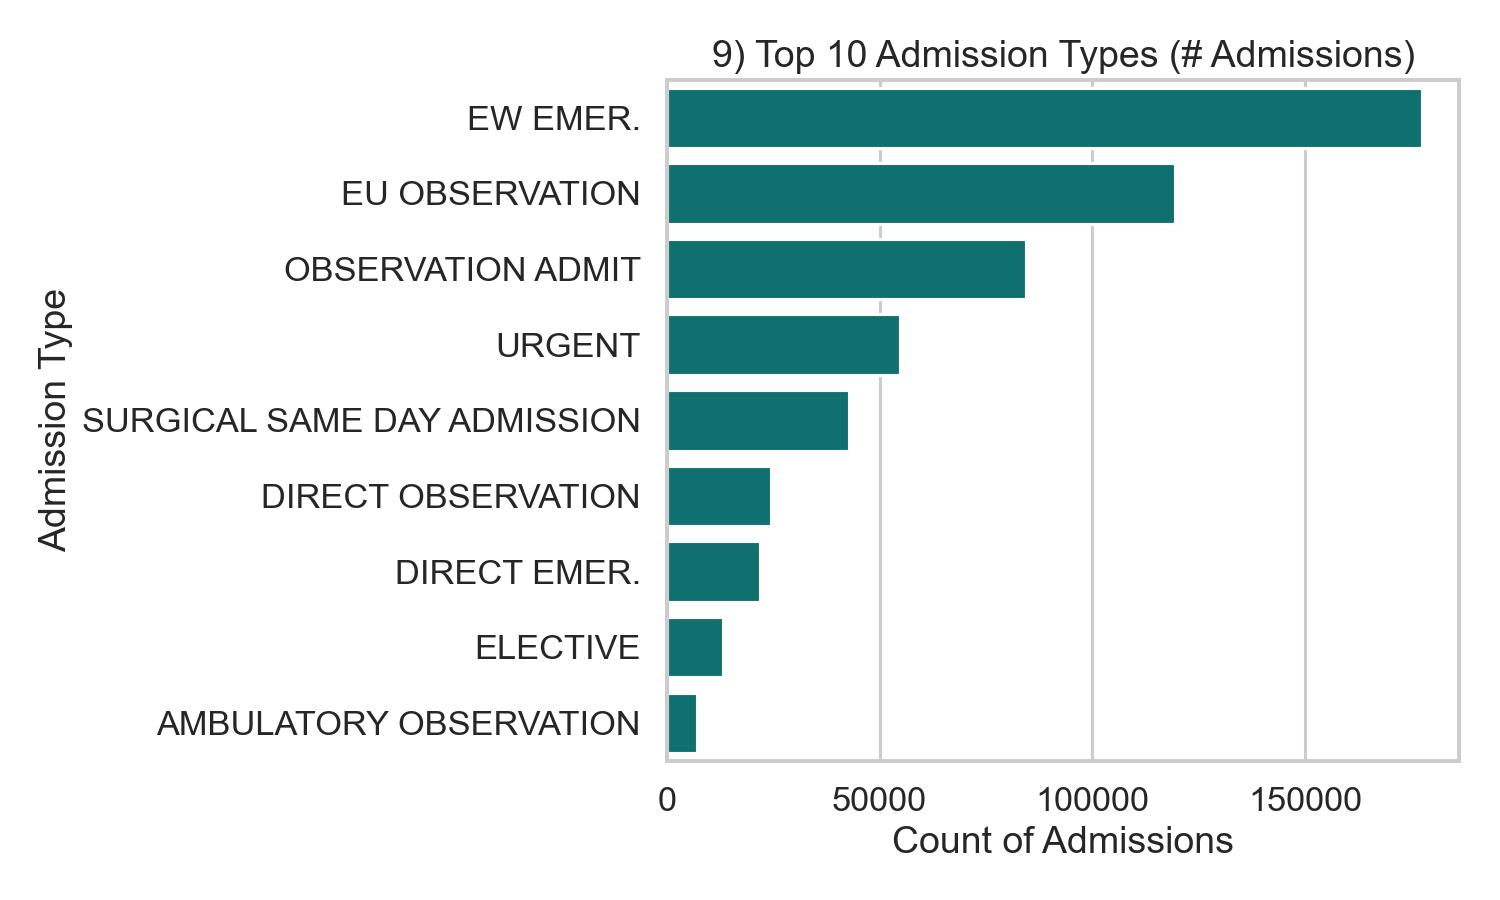
\includegraphics[width=\linewidth]{mimic_plots/plot9.jpg}
    \end{subfigure}\hfill
    \begin{subfigure}{0.54\textwidth}
        \footnotesize
        \textbf{(9) Top 10 Admission Types (\# Admissions)}\newline
        1) A horizontal bar ranking the most frequent admission types.\newline
        2) “EW EMER.” (Emergency) is the largest slice of admissions.\newline
        3) “AMBULATORY OBSERVATION” ranks lowest among the top 10 but is still substantial.
    \end{subfigure}
    \caption{Left: Bar plot of top 10 admission types by volume. Right: Description.}
    \label{fig:plot9}
\end{figure}

\begin{figure}[ht!]
    \centering
    \begin{subfigure}{0.42\textwidth}
        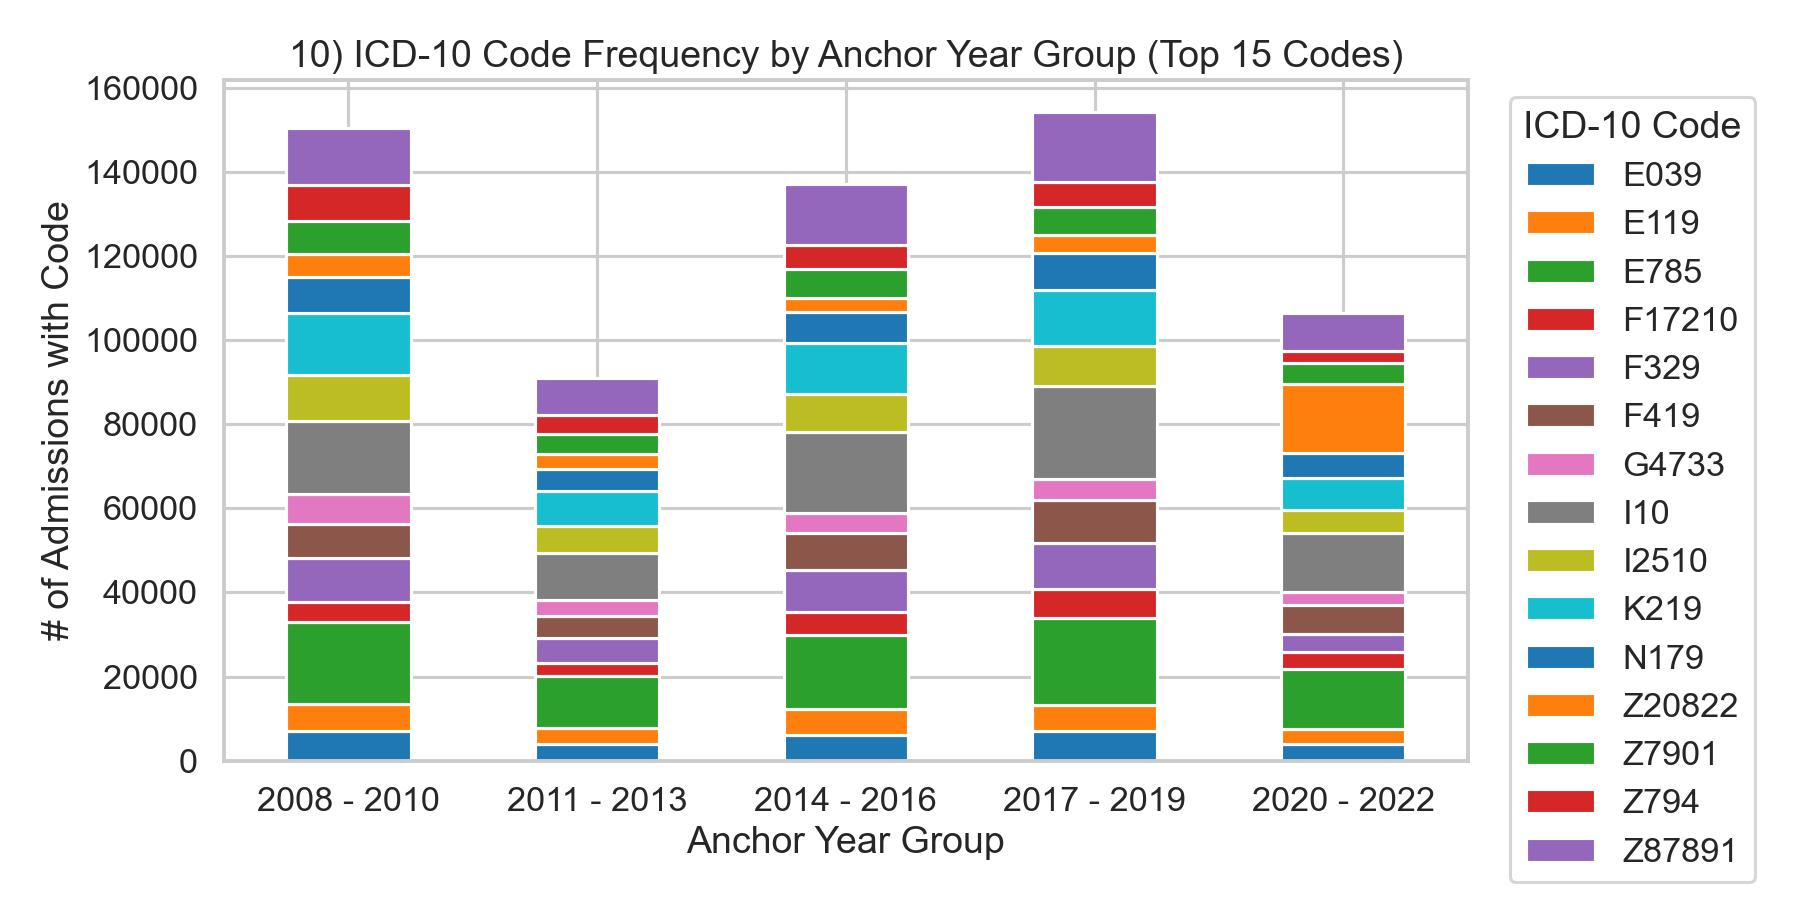
\includegraphics[width=\linewidth]{mimic_plots/plot10.jpg}
    \end{subfigure}\hfill
    \begin{subfigure}{0.54\textwidth}
        \footnotesize
        \textbf{(10) ICD-10 Code Frequency by Anchor Year Group (Top 15 Codes)}\newline
        1) Stacked bars show how often each top-15 ICD-10 code appears per year group.\newline
        2) E785 (hyperlipidemia), I10 (hypertension) remain high across time.\newline
        3) Overall bar heights reflect total admissions with any of these codes in that period.
    \end{subfigure}
    \caption{Left: Stacked bar of top-15 codes across anchor year groups. Right: Description.}
    \label{fig:plot10}
\end{figure}

\section{Key Observations and Implications}
These queries and figures reveal:
\begin{itemize}
    \item \textbf{High Volume of Data:} Over 364k patients and 546k admissions, with \(\sim331k\) discharge summaries available.
    \item \textbf{ICD-10 Emphasis:} \(\sim3.46\)M ICD-10 code assignments vs. \(\sim2.91\)M ICD-9, aligning with modern coding practices.
    \item \textbf{Long-Tailed Codes:} Over 9k ICD-10 codes have fewer than 5 occurrences, underscoring the challenge of rare labels.
    \item \textbf{Multiple Codes per Admission:} An average of 13.6 ICD-10 codes assigned per stay, reflecting a \textit{multi-label} classification problem.
    \item \textbf{Varied Note Lengths:} Discharge summaries range from hundreds to thousands of words, with the top 1\% exceeding 4k words.
\end{itemize}

\section{Final Data Preparation}
\label{sec:final-data-prep}

In order to build a dataset suitable for a scenario akin to AWS Comprehend Medical—where arbitrary clinical text is processed to extract ICD-10-CM codes—we create a single table merging the free-text discharge notes (\texttt{discharge}) with billed ICD diagnoses (\texttt{diagnoses\_icd}), excluding extra demographic fields. This configuration ensures our final text column closely reflects “real world” input, where no additional metadata beyond the raw narrative is guaranteed. 

Concretely, for each hospitalization (\texttt{hadm\_id}), we produce:
\begin{itemize}
    \item A column \texttt{notes}, containing the \textit{unmodified} discharge summary text. 
    \item A column \texttt{icd\_codes}, which is a comma-separated list of all ICD-10-CM codes assigned to that admission.
\end{itemize}

\noindent \textbf{SQL Query:}
\begin{verbatim}
DROP TABLE IF EXISTS mimic.full_notes_with_codes;

CREATE TABLE mimic.full_notes_with_codes AS
SELECT
    d.subject_id,
    d.hadm_id,
    d.text AS notes,
    STRING_AGG(di.icd_code, ',') AS icd_codes
FROM mimic.discharge AS d
JOIN mimic.admissions AS a
  ON d.subject_id = a.subject_id
    AND d.hadm_id = a.hadm_id
JOIN mimic.patients AS p
  ON p.subject_id = d.subject_id
JOIN mimic.diagnoses_icd AS di
  ON di.subject_id = d.subject_id
    AND di.hadm_id = d.hadm_id
WHERE di.icd_version = 10  -- focusing on ICD-10-CM codes only
GROUP BY
    d.subject_id,
    d.hadm_id,
    d.text;
\end{verbatim}


\noindent This final table is readily suitable for a text-to-multilabel model that ingests the discharge narrative in \texttt{notes} and predicts \texttt{icd\_codes}, aligning closely with the use case of free-text medical coding systems.




\chapter{Methodology}

This chapter outlines our comprehensive methodology for automating the prediction of ICD-10-CM codes from clinical texts. Building on insights from recent critical reviews (e.g., \cite{edin2023automated,nguyen2023mimicivicd}) and best practices identified in our literature survey, we propose a stepwise approach that starts with simpler baselines and culminates in advanced retrieval-augmented and knowledge graph (KG)–integrated methods. Our overarching goals are to:

\begin{enumerate}
    \item Ensure a \textbf{fair and reproducible comparison} among all approaches by using consistent data splits and unified evaluation protocols,
    \item \textbf{Address the long-tail distribution} of ICD codes and the associated performance drop for rare labels,
    \item Integrate \textbf{modern deep learning architectures} (e.g., PLM-ICD, ModernBERT) that can handle longer clinical notes,
    \item Investigate the effect of \textbf{retrieval-augmented generation} (RAG) and \textbf{ontology/knowledge graph integration} in improving coverage and interpretability.
\end{enumerate}

\section{Data Preparation and Exploration}

\subsection{Data Sources and Scope}
We focus primarily on:
\begin{itemize}
    \item \textbf{MIMIC-IV} (v2.2 or newer) for real-world discharge summaries annotated with ICD-9 or ICD-10 codes. We concentrate on ICD-10-coded admissions for our main experiments, following recent recommendations \cite{edin2023automated}.
    \item If resources allow, we may also incorporate \textbf{eICU} data or \textbf{synthetic data} (e.g., via JonSnowLabs) to bolster rare-code examples.
\end{itemize}
All data is \textbf{de-identified} to comply with privacy regulations (HIPAA, etc.).

\subsection{Development Environment and Data Processing}
\begin{itemize}
    \item \textbf{Database Tools}: We load \texttt{notes} and \texttt{diagnoses\_icd} (plus relevant admission data) into \textbf{DuckDB} for fast in-memory SQL queries and merges.
    \item \textbf{Cleaning and Normalization}:
    \begin{enumerate}
        \item Remove or redact explicit PHI placeholders.
        \item Convert text to lowercase; optionally retain digits (some studies found removing them hinders certain code predictions).
        \item Tokenize via spaCy or WordPiece (depending on the final model choice).
    \end{enumerate}
    \item \textbf{Data Versioning}: Use Data Version Control (\texttt{DVC}) to track dataset transformations and maintain reproducibility.
\end{itemize}

\subsection{Train/Dev/Test Splits and Stratification}
Following \cite{edin2023automated}, we:
\begin{itemize}
    \item Construct a \textbf{“clean” MIMIC-IV ICD-10} split that minimizes missing codes in the test set.
    \item Remove codes with very few appearances (e.g., fewer than 10).
    \item Apply \textbf{multi-label stratified sampling} to ensure that each code is represented across train/dev/test and that no patient appears in more than one split.
\end{itemize}
This prevents artificially low macro-F1 scores caused by codes not present in the test set.

\subsection{Data Exploration and Analysis}
\begin{itemize}
    \item Create \textbf{code frequency plots} to confirm the severe long-tail distribution.
    \item Consider top-50 or top-200 code subsets for some experiments (allowing more direct comparisons with prior works).
    \item Optionally segment notes (e.g., extracting “History of Present Illness” or “Medications” sections) if needed to reduce noise or standardize input length.
\end{itemize}


\section{Incremental Experiment Design}

To systematically evaluate improvements and control complexity, we propose a four-stage experiment setup:

\subsection{Stage A: Baseline Multi-Label Methods}
\paragraph{Objective:} Provide naive references for multi-label classification of ICD codes.

\begin{itemize}
    \item \textbf{Models}:
    \begin{enumerate}
        \item \textbf{Logistic Regression} (binary relevance): Convert each note to TF-IDF vectors; train one logistic classifier per code.
        \item \textbf{Support Vector Machine} (binary relevance): Similar pipeline, but with linear SVMs.
        \item \textbf{(Optional) KNN} for completeness, though likely inefficient.
    \end{enumerate}
    \item \textbf{Data Variants}:
    \begin{itemize}
        \item Unbalanced dataset (all codes) vs. balanced approaches (oversampling or undersampling).
        \item Possibly top-50 / top-200 codes if needed.
    \end{itemize}
    \item \textbf{Implementation}:
    \begin{itemize}
        \item Use scikit-learn with up to 20k features from TF-IDF for manageability.
        \item Evaluate on micro-F1, macro-F1 (corrected), and perhaps Precision@k to see ranking performance.
    \end{itemize}
\end{itemize}


\subsection{Stage B: Advanced Deep Architectures}
\paragraph{Objective:} Compare popular CNN/RNN/Transformer architectures under a unified training regimen.

\begin{enumerate}
    \item \textbf{Candidates}:
    \begin{itemize}
        \item \textbf{CAML, MultiResCNN, LAAT} \cite{mullenbach2018explainable,li2020multi,vu2020label} with label-wise attention.
        \item \textbf{PLM-ICD} \cite{huang2022plm}, which uses BERT-based embeddings in chunks.
        \item \textbf{ModernBERT} (long context capacity) to handle entire notes if feasible.
    \end{itemize}
    \item \textbf{Training Consistency}:
    \begin{itemize}
        \item All models trained up to 20--30 epochs with \textbf{AdamW}, using warm-up + linear decay for learning rate.
        \item Documents truncated or chunked to 2k--4k tokens (CNN/RNN limit). For ModernBERT, attempt up to 8k tokens.
        \item Decision boundary tuned on the dev set for maximum micro-F1.
    \end{itemize}
    \item \textbf{Outcome}:
    \begin{itemize}
        \item Identify the top-1 or top-2 neural architectures by macro-F1, coverage of rare codes, and interpretability potential.
    \end{itemize}
\end{enumerate}


\subsection{Stage C: RAG + Knowledge Graph Integration}
\paragraph{Objective:} Integrate external knowledge to improve coverage and handle rare/ambiguous codes. \textbf{Apply only to the top models from Stage B} to avoid excessive combinatorial overhead.

\subsubsection{RAG Methods}
\begin{itemize}
    \item \textbf{Retrieval Corpus}: PubMed or in-hospital knowledge base. Pre-encode with a neural retriever (e.g., Sentence-BERT).
    \item \textbf{Integration}:
    \begin{itemize}
        \item For each note, retrieve top-$k$ relevant passages, then either (a) concatenate or (b) late-fuse them in the final encoder.
    \end{itemize}
    \item \textbf{Comparison}:
    \begin{itemize}
        \item Evaluate how RAG affects rare-code recall, code coverage, and never-predicted rates.
    \end{itemize}
\end{itemize}

\subsubsection{Knowledge Graph (KG) Integration}
\begin{itemize}
    \item \textbf{Ontology Mapping}: Map recognized medical entities to SNOMED CT or UMLS IDs.
    \item \textbf{Integration Strategy}:
    \begin{enumerate}
        \item \textbf{Feature Concatenation}: Attach KG-based embeddings to each token or note-level embedding.
        \item \textbf{GNN or Hyperbolic Embeddings}: If feasible, build a small subgraph for each note and aggregate representations, following \cite{ren2022hicu}.
    \end{enumerate}
    \item \textbf{Outcome}:
    \begin{itemize}
        \item Test whether explicit symbolic knowledge helps disambiguate near-duplicate or numeric-based codes.
    \end{itemize}
\end{itemize}

\subsubsection{Combined RAG + KG (Optional)}
If resources allow, we can combine retrieval-augmented text with KG-based features for a “full synergy” pipeline. This is a stretch goal but could yield deeper coverage of rare codes.

\subsection{Stage D: Interpretability and Error Analysis}
\paragraph{Objective:} Provide actionable insights on model decisions and highlight rare-code performance.

\begin{itemize}
    \item \textbf{Attention Visualization}: For CAML or LAAT, highlight which text segments triggered each code.
    \item \textbf{Gradient-based Methods}: On a sample of notes, use SHAP or Integrated Gradients to see if the top model’s rationale is clinically coherent.
    \item \textbf{Error Profiling for Rare Codes}: Evaluate which codes remain never predicted, or incorrectly predicted. Explore how many improved with data augmentation or KG features.
\end{itemize}


\section{Model Training and Evaluation}

\subsection{Loss Functions and Decision Thresholding}
\begin{itemize}
    \item \textbf{Binary Cross Entropy} or \textbf{Focal Loss} are used for multi-label classification in neural models.
    \item Decision threshold is tuned on the dev set to maximize \textbf{micro-F1}.
\end{itemize}

\subsection{Evaluation Metrics}
\begin{enumerate}
    \item \textbf{Micro-F1} and \textbf{Macro-F1 (corrected)}: Avoid penalizing codes absent in test splits.
    \item \textbf{Precision@k} and \textbf{Recall@k}: For top-k predicted codes.
    \item \textbf{Never-Predicted Rate (NPR)}: Fraction of codes the model never outputs correctly.
    \item \textbf{Exact Match Ratio (EMR)} (optional): Proportion of notes for which the predicted set of codes is exactly correct.
\end{enumerate}
We additionally track improvements on rare codes specifically, e.g., by computing macro-F1 restricted to codes with fewer than $M$ training examples.




\section{Plan}

This chapter presents a comprehensive plan for analyzing and preparing the MIMIC-IV dataset before building our automated ICD coding framework. It outlines the key questions, steps, and considerations essential for understanding and structuring the data. The subsequent “Implementation” section will detail the practical execution of this plan.

\subsection{Overview of MIMIC-IV}

\paragraph{Motivation and Context.}
MIMIC-IV is a large, de-identified database that combines critical care records from the Beth Israel Deaconess Medical Center (BIDMC). It contains extensive information about patient hospitalizations, including demographics, physiological measurements, clinical notes, and administrative data. The dataset is a cornerstone for machine learning and data science research in healthcare, especially for tasks such as mortality prediction, readmission risk assessment, and—as in our project—automated ICD coding.

\paragraph{Module Structure.}
MIMIC-IV is partitioned into multiple modules:
\begin{itemize}
  \item \textbf{hosp}: Hospital-wide data (demographics, admissions, diagnoses, procedures, etc.).
  \item \textbf{icu}: ICU-specific data (high-frequency chart events, procedures, inputs/outputs).
  \item \textbf{ed}: Data from the emergency department.
  \item \textbf{note}: Textual notes, including discharge summaries and radiology reports.
  \item \textbf{cxr}: Linking data for chest X-ray images (MIMIC-CXR), if used.
\end{itemize}
For automated ICD coding from discharge summaries, our core focus is on:
\begin{itemize}
  \item \texttt{diagnoses\_icd} (in the \emph{hosp} module),
  \item \texttt{admissions} (in the \emph{hosp} module),
  \item \texttt{patients} (in the \emph{hosp} module), and
  \item \texttt{discharge} notes (in the \emph{note} module).
\end{itemize}
Nonetheless, we keep open the possibility of integrating ICU or ED data for additional features if required.

\subsection{Data Characteristics and Key Questions}

\subsubsection{Patient Population and Diversity}
\begin{itemize}
    \item \textbf{Size and Composition.} The dataset includes over 40,000 patients, spanning a broad demographic range. We need to confirm how these patients are distributed across different age groups, gender, and anchor-year cohorts.
    \item \textbf{Clinical Relevance.} Because many patients in MIMIC-IV are in critical care, the dataset may have disease distributions that differ from general hospital populations. We ask: \emph{Does this skew limit generalizability for ICD coding?}
\end{itemize}

\subsubsection{Hospital Admissions and ICD Codes}
\begin{itemize}
    \item \textbf{Admissions Volume.} Each admission is uniquely identified by \texttt{hadm\_id}, and some patients have multiple admissions. We plan to analyze the average number of admissions per patient.
    \item \textbf{ICD Code Assignments.} Diagnoses in MIMIC-IV are stored in \texttt{diagnoses\_icd}, which includes both ICD-9 and ICD-10 codes. We must identify how many admissions have ICD-10 codes, how many distinct codes appear, and the frequency distribution (long-tailed phenomenon).
    \item \textbf{Rare Code Challenge.} A key question is how many ICD codes appear fewer than, say, 10 or 20 times. We hypothesize a large fraction of codes are rare, which complicates classification.
\end{itemize}

\subsubsection{Discharge Summaries}
\begin{itemize}
    \item \textbf{Text Volume and Lengths.} Over 330,000 unique clinical notes exist, and many are discharge summaries with an average of about 1,500 words. We plan to measure the actual length distribution (e.g., short vs. very long notes).
    \item \textbf{Free-Text Complexity.} Clinical narratives often include abbreviations, domain-specific jargon, and redundancies (colloquially “note bloat”). We want to see if we need advanced text preprocessing or chunking for our modeling.
    \item \textbf{Linking to ICD Codes.} The discharge summaries are linked to \texttt{admissions} and \texttt{diagnoses\_icd} by \texttt{subject\_id} and \texttt{hadm\_id}. We must verify we can retrieve a consistent set of (note, ICD codes) pairs for each admission.
\end{itemize}

\subsection{Data Preprocessing Plan}

\paragraph{1) Data Extraction and Joining.}
We plan to retrieve the relevant columns from:
\begin{itemize}
    \item \texttt{admissions}: (\texttt{hadm\_id}, \texttt{subject\_id}, \texttt{admittime}, \texttt{dischtime}, etc.)
    \item \texttt{diagnoses\_icd}: (\texttt{subject\_id}, \texttt{hadm\_id}, \texttt{icd\_code}, \texttt{icd\_version})
    \item \texttt{discharge}: (\texttt{subject\_id}, \texttt{hadm\_id}, \texttt{text} of the summary)
    \item \texttt{patients}: (\texttt{subject\_id}, \texttt{anchor\_age}, \texttt{anchor\_year\_group}, \texttt{gender})
\end{itemize}
We will join them into a consolidated “analysis-ready” dataset, making sure we do not lose admissions that lack a discharge summary or lack ICD codes (the plan is to see if they are relevant or must be discarded).

\paragraph{2) Text Cleaning.}
Discharge summaries will be processed to:
\begin{itemize}
    \item Remove PHI placeholders such as \texttt{[\*\*...\*\*]} strings.
    \item Optionally convert to lowercase and handle special characters.
    \item Tokenize and segment into sections (e.g., “History of Present Illness,” “Medications,” etc.) if beneficial for more structured modeling.
\end{itemize}
We will pay special attention to the presence of numerical data or standard medical abbreviations that might be relevant to ICD coding.

\paragraph{3) Handling Missing or Inconsistent Entries.}
\begin{itemize}
    \item \textbf{No Discharge Summary.} Some admissions may not have a final discharge summary (e.g., if the patient expired quickly in the ED). Decide whether to drop or keep them.
    \item \textbf{No ICD Codes.} Some admissions might lack coded diagnoses (or have only ICD-9 codes). We are focusing on ICD-10-coded admissions, so these will likely be excluded from training data.
\end{itemize}

\paragraph{4) Dealing with Duplicates and Similar Notes.}
Clinical notes can be duplicated or near-duplicated (e.g., discharge summary repeated in an addendum). We plan to:
\begin{itemize}
    \item Apply LSH/MinHash or a similar approach to identify near-duplicates.
    \item Decide how to treat duplicates (either remove or unify) to avoid artificially inflating training data.
\end{itemize}

\subsection{Data Imbalance Considerations}

\paragraph{1) Code Frequency Distribution.}
After joining notes with ICD codes, we will plot the frequency distribution of codes to confirm the expected heavy-tail phenomenon. Identifying how many codes occur below certain frequency thresholds (e.g., 10 or 20) is crucial for modeling decisions.

\paragraph{2) Augmentation Strategy.}
We aim to use Retrieval-Augmented Generation (RAG) or knowledge-based approaches to generate synthetic notes for rare codes. We need to:
\begin{itemize}
    \item Identify which codes are “rare enough” to warrant synthetic data generation.
    \item Validate synthetic data qualitatively and quantitatively.
\end{itemize}

\subsection{Data Storage and Management Plan}

\paragraph{Database: DuckDB.}
We have decided to use DuckDB for:
\begin{itemize}
    \item \textbf{In-Memory Efficiency}: Facilitates fast prototyping and interactive queries on structured MIMIC-IV data.
    \item \textbf{Easy Integration with Python}: We can use standard Python scripts (pandas, Polars, or pyduckdb) to manipulate large tables.
\end{itemize}

\paragraph{Scalability.}
As we add synthetic data or additional external knowledge bases (e.g., SNOMED CT lookups), we must ensure our data pipeline can handle the expanded volume. DuckDB’s columnar design should suffice for pilot experiments, but we may move to a larger-scale database if needed.

\paragraph{Version Control.}
All transformations—SQL queries, Python data merges, and text cleaning scripts—will be tracked by Data Version Control (DVC) or Git to ensure reproducibility.

\subsection{Security and Compliance}

\paragraph{De-Identification.}
MIMIC-IV is already de-identified, but we must confirm no re-identification can occur, especially after generating synthetic notes. We will:
\begin{itemize}
    \item Double-check that any new outputs or textual data do not inadvertently reveal PII.
    \item Use safe text generation protocols for synthetic data augmentation.
\end{itemize}

\paragraph{Regulatory Aspects.}
We comply with HIPAA standards and adhere to the data use agreement set forth by PhysioNet for MIMIC-IV. Any derivative dataset (e.g., synthetic expansions) must remain under the same data usage constraints.

\subsection{Summary of the Plan}
In summary, our plan is to:
\begin{enumerate}
    \item Thoroughly \textbf{join and explore} the relevant tables (admissions, patients, diagnoses, discharge).
    \item \textbf{Clean and standardize} the discharge summaries, paying attention to near-duplicates and missing data.
    \item \textbf{Quantify the code imbalance} to identify “rare codes” that require augmentation.
    \item \textbf{Adopt a robust data management} workflow (DuckDB + version control) for reproducibility.
    \item Maintain strict \textbf{compliance and ethical guidelines}.
\end{enumerate}
The final outcome is an “analysis-ready” table linking each admission (hadm\_id) to a single discharge summary text and a set of ICD-10 codes for supervised learning.

\section{Implementation (Planned)}

\textbf{[TODO: This section will be filled after we execute the plan. Below is a high-level outline of anticipated steps:]} 

\begin{enumerate}
    \item \textbf{Data Loading (SQL + Python)}  
    We will load the CSV or Parquet files for \texttt{admissions}, \texttt{diagnoses\_icd}, \texttt{patients}, and \texttt{discharge} into DuckDB. Example pseudo-code:
\begin{verbatim}
CREATE TABLE admissions AS
  SELECT * FROM 'admissions.csv';

CREATE TABLE diagnoses_icd AS
  SELECT * FROM 'diagnoses_icd.csv';

CREATE TABLE discharge AS
  SELECT * FROM 'discharge.csv';
...
\end{verbatim}
    \item \textbf{Data Joining and Filtering}  
    - Use \texttt{JOIN} on \texttt{subject\_id} and \texttt{hadm\_id} to link discharge summaries to diagnoses.  
    - Filter out non-ICD-10 codes or admissions without discharge summaries.  
    - Keep only rows that satisfy minimal length or minimal code frequency conditions.

    \item \textbf{Text Preprocessing and Deduplication}  
    - Python scripts to remove PHI placeholders, convert to lowercase, and tokenize.  
    - MinHash-based duplication check, removing or merging near-identical summaries.

    \item \textbf{Statistical Summaries and Visualizations}  
    - Generate histograms of note lengths.  
    - Plot ICD code frequencies in log scale to confirm data imbalance.  

    \item \textbf{Integration with Ontologies / Knowledge Graphs}  
    - If needed, for each token or concept recognized, map to UMLS or SNOMED CT identifiers for advanced features.  
    - Store these mappings in auxiliary tables for easy joining.

    \item \textbf{Version Control and Outputs}  
    - Use DVC or Git for each transformation script to allow rollback and reproducibility.  
    - Produce final “analysis-ready” table(s) stored in DuckDB or CSV with columns: \texttt{subject\_id, hadm\_id, discharge\_text, [list of ICD-10 codes]}.
\end{enumerate}

Once these tasks are completed, we will have a clean, joined, and labeled dataset suitable for training and evaluating our ICD coding models. The subsequent chapters will detail how these data products feed into the modeling pipeline and how synthetic data augmentation is integrated. 







\chapter{Results}

\section{Baseline Model Experiments}

\subsection{K-Nearest Neighbors (KNN) Classifier}
\begin{itemize}
    \item \textbf{Objective}: Establish a baseline for multi-label ICD code prediction using simple models.
    \item \textbf{Methodology}:
    \begin{itemize}
        \item \textbf{Text Vectorization}: Used TF-IDF vectorizer with a maximum of 5,000 features and n-gram range of (1,2).
        \item \textbf{Multi-Label Binarization}: Applied \textbf{MultiLabelBinarizer} to handle multiple ICD codes per clinical note.
        \item \textbf{Model Training}: Trained a KNN classifier on the vectorized text data.
    \end{itemize}
    \item \textbf{Results}:
    \begin{itemize}
        \item \textbf{Evaluation Metrics}: Used Hamming Loss and Macro F1-Score to assess performance.
        \item \textbf{Performance}: The model achieved a Macro F1-Score of 0.12, indicating poor performance, especially on rare codes.
        \item \textbf{Analysis}: High Hamming Loss and low F1-Score confirmed that the model struggled with data imbalance and text complexity.
    \end{itemize}
\end{itemize}

\subsection{Observations}
\begin{itemize}
    \item The baseline model highlighted the challenges in predicting ICD codes using traditional machine learning approaches.
    \item Reinforced the need for advanced models that can handle complex clinical texts and data imbalance.
\end{itemize}

\section{Similarity Matching Using MinHash}

\subsection{Objective}
Identify duplicate or highly similar clinical notes to reduce redundancy and potentially improve model training.

\subsection{Methodology}
\begin{itemize}
    \item \textbf{Text Preprocessing}: Applied standard preprocessing steps to clean the text.
    \item \textbf{MinHash and LSH}: Used MinHash to create signatures for each document and Locality Sensitive Hashing (LSH) to efficiently identify similar documents.
    \item \textbf{Threshold Setting}: Set similarity thresholds (e.g., 90\% and 97\%) to identify pairs of similar notes.
\end{itemize}

\subsection{Results}
\begin{itemize}
    \item Identified 260 notes with over 90\% similarity.
    \item Found six notes with over 97\% similarity, indicating nearly identical content.
    \item Verification with a medical expert confirmed that these notes were indeed similar or duplicates.
\end{itemize}

\subsection{Implications}
\begin{itemize}
    \item Removing or consolidating similar notes can reduce data redundancy.
    \item May improve model performance by preventing the model from being biased towards duplicated information.
\end{itemize}

\section{Challenges Identified}
\begin{itemize}
    \item \textbf{Data Imbalance}: The initial models confirmed that frequent codes dominate predictions, and rare codes are often missed.
    \item \textbf{Model Limitations}: Simple models like KNN are insufficient for capturing the complexity of clinical narratives.
    \item \textbf{Need for Advanced Techniques}: Emphasized the importance of implementing transformer-based models and data augmentation strategies.
\end{itemize}

\chapter{Conclusion and Work Timeline}

\section{Summary of Work}
In the initial phase of this project, we have:
\begin{itemize}
    \item Established a robust development environment with appropriate tools and infrastructure.
    \item Explored and acquired various datasets and medical knowledge graphs to support data augmentation and knowledge integration.
    \item Conducted data exploration and preprocessing, including identifying redundant clinical notes.
    \item Implemented baseline models to understand the challenges in predicting ICD codes.
    \item Identified key challenges such as data imbalance, complexity of clinical texts, and the limitations of traditional machine learning models.
\end{itemize}

\section{Future Work}
Moving forward, the following tasks are planned:

\subsection{Phase 1: Data Augmentation (Months 3-5)}
\begin{itemize}
    \item Implement hybrid data augmentation techniques combining RAG and ontology-based methods.
    \item Generate synthetic clinical notes for rare ICD codes to balance the dataset.
    \item Validate the quality of synthetic data with clinical experts.
\end{itemize}

\subsection{Phase 2: Transformer-Based Model Development (Months 5-7)}
\begin{itemize}
    \item Develop and fine-tune transformer-based models suitable for long clinical documents.
    \item Integrate knowledge graph embeddings to enhance the model's understanding of medical concepts and relationships.
    \item Address computational challenges by optimizing model architectures and training procedures.
\end{itemize}

\subsection{Phase 3: Model Training and Evaluation (Months 7-8)}
\begin{itemize}
    \item Train the model using the augmented dataset.
    \item Evaluate performance using appropriate metrics, focusing on rare code prediction.
    \item Perform error analysis to identify areas for improvement.
\end{itemize}

\subsection{Phase 4: Explainability Integration (Months 8-9)}
\begin{itemize}
    \item Integrate explainability techniques to provide interpretable predictions.
    \item Develop visualization tools for presenting explanations to clinicians.
    \item Gather feedback from healthcare professionals to refine explanations.
\end{itemize}

\subsection{Phase 5: Deployment and Validation (Months 9-10)}
\begin{itemize}
    \item Deploy the model as an open-source toolkit.
    \item Validate the model with clinician feedback and refine as necessary.
    \item Document the methodology and results for publication.
\end{itemize}

\section{Timeline}
\begin{figure}[H]
    \centering
    \begin{ganttchart}[
        hgrid,
        vgrid,
        x unit=0.7cm,
        y unit title=0.6cm,
        y unit chart=0.6cm,
        title height=1,
        bar/.style={fill=blue!50},
        bar height=0.5
    ]{1}{11}
        \gantttitle{Project Timeline (Months)}{11} \\
        \gantttitlelist{1,...,11}{1} \\
        \ganttbar{Phase 1: Data Augmentation}{3}{5} \\
        \ganttbar{Phase 2: Model Development}{5}{7} \\
        \ganttbar{Phase 3: Training and Evaluation}{7}{8} \\
        \ganttbar{Phase 4: Explainability Integration}{8}{9} \\
        \ganttbar{Phase 5: Deployment \& Validation}{9}{10} \\
    \end{ganttchart}
    \caption{Gantt Chart of Planned Work Timeline}
\end{figure}

\section{Potential Challenges and Contingency Plans}
\begin{itemize}
    \item \textbf{Computational Resources}: If computational limitations arise, we will explore cloud-based solutions or optimize model architectures for efficiency.
    \item \textbf{Data Quality}: In case synthetic data does not sufficiently improve model performance, we will consider alternative data augmentation techniques or focus on enhancing model robustness.
    \item \textbf{Model Interpretability}: If explainability methods do not meet clinician requirements, we will investigate other interpretability frameworks or simplify the model for better transparency.
\end{itemize}

\section{Concluding Remarks}
This thesis aims to contribute to the field of automated ICD coding by addressing critical challenges through innovative methods. By combining hybrid data augmentation, advanced modeling techniques, and explainability, we anticipate improving prediction accuracy, particularly for rare ICD codes, and enhancing the usability of automated coding systems in clinical settings. The successful completion of this project could pave the way for further applications of data augmentation and knowledge integration in medical NLP tasks.


\begin{thebibliography}{99}

\bibitem{who2019icd11}
World Health Organization.
\newblock \emph{International Classification of Diseases 11th Revision (ICD-11)}.
\newblock 2019.

\bibitem{dong2022automated}
Dong, H., Su\'arez-Paniagua, V., Whiteley, W., \& Wu, H.
\newblock Automated clinical coding: what, why, and where we are?
\newblock \emph{npj Digital Medicine}, 5, 159, 2022.

\bibitem{edin2023automated}
Edin, J., Jensen, S.~M., Sahlgren, M., L{\"o}vgren, J., \& Henriksson, A.
\newblock Automated medical coding on MIMIC-III and MIMIC-IV: a critical review and replicability study.
\newblock In \emph{Proceedings of the 46th International ACM SIGIR Conference on Research and Development in Information Retrieval}, 2023.

\bibitem{farkas2008automatic}
Farkas, R. \& Szarvas, G.
\newblock Automatic construction of rule-based ICD-9-CM coding systems.
\newblock \emph{BMC Bioinformatics}, 9(1), 2008.

\bibitem{scheurwegs2017data}
Scheurwegs, E., Luyckx, K., Luyten, L., \& Daelemans, W.
\newblock Data integration of structured and unstructured sources for assigning clinical codes to patient stays.
\newblock \emph{Journal of the American Medical Informatics Association}, 24(e1):e68--e76, 2017.

\bibitem{perotte2014diagnosis}
Perotte, A., Wood, F., Simma, A., Braverman, M., Elhadad, N., \& Ghosh, S.
\newblock Diagnosis code assignment: models and evaluation metrics.
\newblock \emph{Journal of the American Medical Informatics Association}, 21(2):231--237, 2014.

\bibitem{lecun2015deep}
LeCun, Y., Bengio, Y., \& Hinton, G.
\newblock Deep learning.
\newblock \emph{Nature}, 521(7553):436--444, 2015.

\bibitem{kim2014convolutional}
Kim, Y.
\newblock Convolutional neural networks for sentence classification.
\newblock In \emph{Proceedings of the 2014 Conference on Empirical Methods in Natural Language Processing (EMNLP)}, pages 1746--1751, 2014.

\bibitem{mullenbach2018explainable}
Mullenbach, J., Wiegreffe, S., Duke, J., Sun, J., \& Eisenstein, J.
\newblock Explainable prediction of medical codes from clinical text.
\newblock In \emph{Proceedings of the 2018 Conference of the North American Chapter of the Association for Computational Linguistics}, pages 1101--1111, 2018.

\bibitem{li2020multi}
Li, F. \& Yu, H.
\newblock ICD coding from clinical text using multi-filter residual convolutional neural network.
\newblock In \emph{Proceedings of the AAAI Conference on Artificial Intelligence}, 34, 8180--8187, 2020.

\bibitem{hochreiter1997long}
Hochreiter, S. \& Schmidhuber, J.
\newblock Long short-term memory.
\newblock \emph{Neural Computation}, 9(8):1735--1780, 1997.

\bibitem{vu2020label}
Vu, T., Nguyen, D.~Q., \& Nguyen, A.
\newblock A label attention model for ICD coding from clinical text.
\newblock \emph{Journal of Biomedical Informatics}, 102:103381, 2020.

\bibitem{devlin2019bert}
Devlin, J., Chang, M.-W., Lee, K., \& Toutanova, K.
\newblock BERT: Pre-training of deep bidirectional transformers for language understanding.
\newblock In \emph{Proceedings of NAACL-HLT}, pages 4171--4186, 2019.

\bibitem{gao2021limitations}
Gao, S., Alawad, M., Young, M.~T., Gounley, J., Schaefferkoetter, N., Yoon, H.~J., et al.
\newblock Limitations of transformers on clinical text classification.
\newblock \emph{IEEE Journal of Biomedical and Health Informatics}, 25(9):3596--3607, 2021.

\bibitem{huang2022plm}
Huang, C.-W., Tsai, S.-C., \& Chen, Y.-N.
\newblock PLM-ICD: Automatic ICD coding with pre-trained language models.
\newblock In \emph{Proceedings of the 4th Clinical Natural Language Processing Workshop}, pages 10--20, 2022.

\bibitem{heo2022medical}
Heo, T.-S., Jo, B., Yoo, Y., Lee, K., Park, Y., \& Kim, K.
\newblock Medical code prediction from discharge summary: Document to sequence BERT using sequence attention.
\newblock In \emph{2022 International Conference on Electronics, Information, and Communication (ICEIC)}, pages 1--4, 2022.

\bibitem{portes2023mosaicbert}
Portes, J., Trott, A., Havens, S., et al.
\newblock MosaicBERT: A bidirectional encoder optimized for fast pretraining.
\newblock \emph{Advances in Neural Information Processing Systems}, 36, 2023.

\bibitem{geiping2023cramming}
Geiping, J. \& Goldstein, T.
\newblock Cramming: Training a language model on a single GPU in one day.
\newblock In \emph{International Conference on Machine Learning}, 2023.

\bibitem{nussbaum2024nomicbert}
Nussbaum, Z., Morris, J.~X., Duderstadt, B., \& Mulyar, A.
\newblock NomicBERT: Training a reproducible long context text embedder.
\newblock \emph{arXiv preprint arXiv:2402.01613}, 2024.

\bibitem{zhang2024gte}
Zhang, X., Zhang, Y., Long, D., \& Xie, W.
\newblock GTE-en-MLM: Generalized long-context text representation for retrieval tasks.
\newblock \emph{Proceedings of the 2024 Conference on Empirical Methods in Natural Language Processing}, 2024.

\bibitem{warner2024modernbert}
Warner, B., Chaffin, A., Clavié, B., et al.
\newblock Smarter, Better, Faster, Longer: A Modern Bidirectional Encoder for Fast, Memory Efficient, and Long Context Finetuning and Inference.
\newblock \emph{arXiv preprint arXiv:2309.16609}, 2024.

\bibitem{bengio2009curriculum}
Bengio, Y., Louradour, J., Collobert, R., \& Weston, J.
\newblock Curriculum learning.
\newblock In \emph{Proceedings of the 26th Annual International Conference on Machine Learning}, pages 41--48, 2009.

\bibitem{ren2022hicu}
Ren, W., Zeng, R., Wu, T., Zhu, T., \& Krishnan, R.~G.
\newblock HiCu: Leveraging hierarchy for curriculum learning in automated ICD coding.
\newblock In \emph{Proceedings of the Machine Learning for Healthcare Conference}, pages 1--24, 2022.

\bibitem{johnson2016mimic}
Johnson, A.~E.~W., Pollard, T.~J., Shen, L., et al.
\newblock MIMIC-III, a freely accessible critical care database.
\newblock \emph{Scientific Data}, 3(160035), 2016.

\bibitem{rios2018few}
Rios, A. \& Kavuluru, R.
\newblock Few-shot and zero-shot multi-label learning for structured label spaces.
\newblock In \emph{Proceedings of the 2018 Conference on Empirical Methods in Natural Language Processing}, pages 3132--3142, 2018.

\bibitem{wrenn2010quantifying}
Wrenn, J.~O., Stein, D.~M., Bakken, S., \& Stetson, P.~D.
\newblock Quantifying clinical narrative redundancy in an electronic health record.
\newblock \emph{Journal of the American Medical Informatics Association}, 17:49--53, 2010.

\bibitem{holzinger2017we}
Holzinger, A., Dehmer, M., \& Jurisica, I.
\newblock What do we need to build explainable AI systems for the medical domain?
\newblock \emph{arXiv preprint arXiv:1712.09923}, 2017.

\bibitem{edin2024unsupervised}
Edin, J., Borgholt, L., Maistro, M., et al.
\newblock An unsupervised approach to achieve supervised-level explainability in healthcare records.
\newblock \emph{arXiv preprint arXiv:2406.08958}, 2024.

\bibitem{teng2020explainable}
Teng, F., Yang, W., Chen, L., Huang, L., \& Xu, Q.
\newblock Explainable prediction of medical codes with knowledge graphs.
\newblock \emph{Frontiers in Bioengineering and Biotechnology}, 8:867, 2020.

\bibitem{xie2019ehr}
Xie, X., Xiong, Y., Yu, P.~S., \& Zhu, Y.
\newblock EHR coding with multi-scale feature attention and structured knowledge graph propagation.
\newblock In \emph{Proceedings of the 28th ACM International Conference on Information and Knowledge Management}, pages 649--658, 2019.

\bibitem{nickel2017poincare}
Nickel, M. \& Kiela, D.
\newblock Poincaré embeddings for learning hierarchical representations.
\newblock In \emph{Advances in Neural Information Processing Systems}, pages 6338--6347, 2017.

\bibitem{kumichev2024medsyn}
Kumichev, G., Blinov, P., Kuzkina, Y., et al.
\newblock MedSyn: LLM-based synthetic medical text generation framework.
\newblock \emph{arXiv preprint arXiv:2408.02056}, 2024.

\bibitem{excoffier2024generalist}
Excoffier, J.-B., Roehr, T., Figueroa, A., Bressem, K., \& Ortala, M.
\newblock Generalist embedding models are better at short-context clinical semantic search than specialized embedding models.
\newblock \emph{arXiv preprint arXiv:2401.01943}, 2024.

\bibitem{campbell2020computer}
Campbell, S. \& Giadresco, K.
\newblock Computer-assisted clinical coding: A narrative review of the literature on its benefits, limitations, implementation, and impact on clinical coding professionals.
\newblock \emph{Health Information Management Journal}, 49(1):5--18, 2020.

\bibitem{kraljevic2021multi}
Kraljevic, Z., Searle, T., Shek, A., et al.
\newblock Multi-domain clinical natural language processing with MedCAT: The medical concept annotation toolkit.
\newblock \emph{Artificial Intelligence in Medicine}, 117:102083, 2021.

\bibitem{gaebel2020changes}
Gaebel, W., Stricker, J., \& Kerst, A.
\newblock Changes from ICD-10 to ICD-11 and future directions in psychiatric classification.
\newblock \emph{Dialogues in Clinical Neuroscience}, 22(1):7--15, 2020.

\bibitem{wang2021meta}
Wang, R., Song, X., Chen, J., et al.
\newblock Meta-LMTC: Meta-learning for large-scale multi-label text classification.
\newblock In \emph{Proceedings of the 2021 Conference on Empirical Methods in Natural Language Processing}, pages 8633--8646, 2021.

\bibitem{nguyen2023mimicivicd}
Nguyen, T.-T., Schlegel, V., Kashyap, A., Winkler, S., Huang, S.-S., Liu, J.-J., \& Lin, C.-J.
\newblock MIMIC-IV-ICD: A new benchmark for extreme multi-label classification.
\newblock In \emph{Proceedings of the 61st Annual Meeting of the Association for Computational Linguistics}, 2023.

\bibitem{johnson2023mimicivscidata}
Johnson, A.~E.~W., Bulgarelli, L., Shen, L., Gayles, A., Shammout, A., Horng, S., Pollard, T.~J., Hao, S., Moody, B., Gow, B., Lehman, L.~H., Celi, L.~A., \& Mark, R.~G.
\newblock MIMIC-IV, a freely accessible electronic health record dataset.
\newblock \emph{Scientific Data}, 10(1):1, 2023.
\newblock \,doi:10.1038/s41597-022-01899-x.

\end{thebibliography}



\end{document}
